\chapter{Implementación}
\label{implementacion}

Hasta ahora, con todas las piezas de información que hemos generado acerca del desarrollo, hemos podido, en efecto, discernir entre tres grandes grupos de tareas: la gestión, el calendario y el panel de control. Así pues, estableceremos la separación del desarrollo en estos tres grandes bloques de trabajo, con la previa especificación de las herramientas a utilizar y del trabajo anterior al comienzo del proceso de programación, propiamente dicho, que implican la puesta a punto de la base de datos y del servidor para probar y desarrollar nuestra aplicación.

\section{Herramientas para el desarrollo de twinX}
\label{sec:herramientasdesarrollo}

Para llevar a cabo la programación de este sitio web, aunque utilicemos herramientas más sofisticadas, éstas están basadas en los clásicos lenguajes web: \textbf{HTML} (\textit{HyperText Markup Language}) \cite{html} para la estructuración de la web y la identificación de los distintos elementos, \textbf{CSS} \cite{css} (\textit{Cascading Style Sheets}) para aplicar estilo a la vista (posicionamiento, colores, visibilidad, etc.) y \textbf{JavaScript} \cite{javascript}, para implementar funciones más complejas a cada componente de la web. Para el manejo de estos dos últimos, contaremos con la ayuda de dos librerías con un gran potencial. Para el estilo, usaremos \textbf{Bootstrap} \cite{bootstrap} en su cuarta versión y para JavaScript utilizaremos \textbf{jQuery} \cite{jquery}. Nos permitirán ahorrar mucho tiempo, ya que en ambos casos podemos hacer uso de funciones o palabras clave que evitarán el tener que escribir numerosas líneas de código en cada uno de los lenguajes a los que complementan.

Como ya hemos mencionado en varias ocasiones, el desarrollo va a ser llevado a cabo con la ayuda de \textbf{Yii2 Framework}\footnote{Sus siglas significan \textit{Yes, it is!}}. En su segunda versión, este framework hace uso del lenguaje de programación PHP para orquestar múltiples tareas que resultan engorrosas de llevar a cabo sin su ayuda y que pueden extenderse demasiado, como son, por ejemplo, las operaciones con la base de datos o la generación de código del que partir para dar forma a la vista, modelo o controlador de alguna de las secciones de twinX \cite{yii}. Hoy en día, en proyectos de desarrollo, sería muy complicado prescindir de una herramienta como esta, ya que las alternativas son numerosas y completas.

Entre sus características, destacamos el generador de código \textbf{Gii} (figura \ref{fig:gii}), que puede automatizar la creación, por ejemplo, de la clase de un modelo, o incluso de una tabla CRUD al completo (es decir, su vista y su controlador). Tan solo tenemos que indicar cuál es la tabla de la base de datos sobre la que queremos generar los fragmentos de código, y atendiendo a las restricciones creadas en la misma, se puede obtener fácilmente una clase instanciable para recuperar o guardar información en su tabla. Del mismo modo, al crear una tabla CRUD, tendríamos directamente en nuestro sitio web una interfaz donde pueden verse los registros almacenados en la base de datos, con la posibilidad de crear nuevos, eliminarlos o incluso filtrarlos y editarlos. No cabe duda del potencial de esta característica, la cual nos permitirá ahorrar mucho tiempo y seguridad a la hora de desarrollar y de depositar la confianza en código automáticamente generado y sin errores.

\begin{figure}
	\centering
	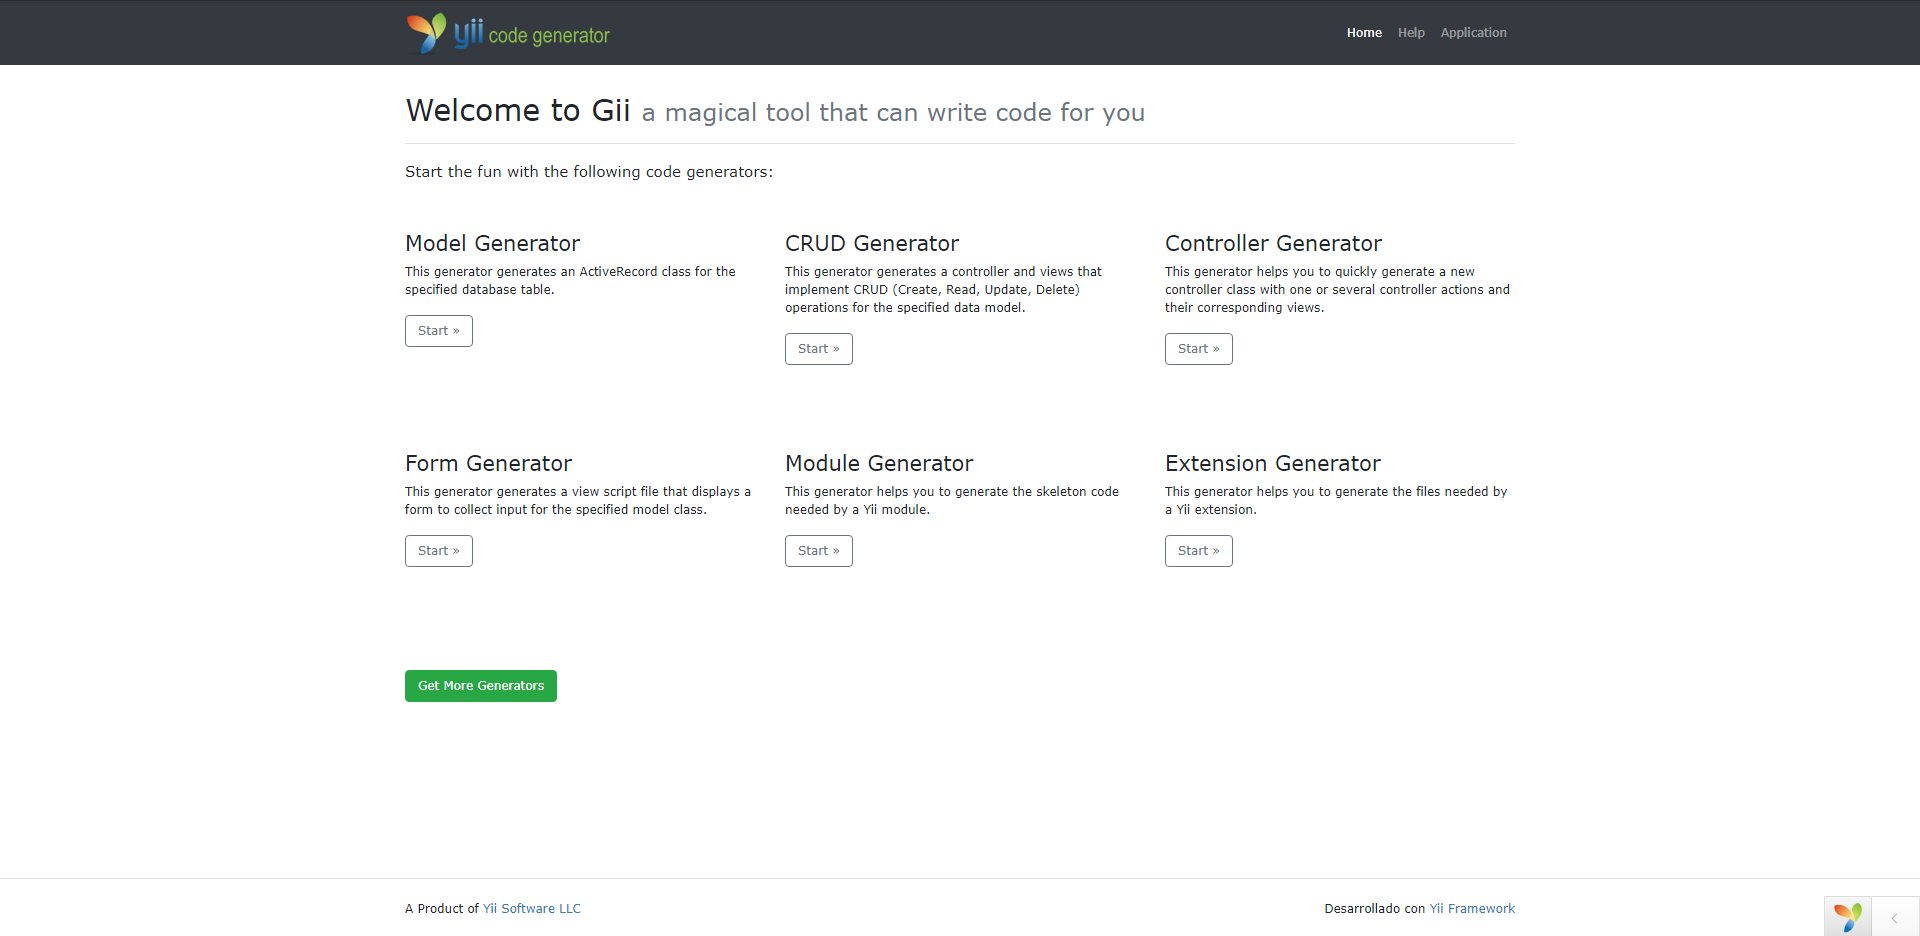
\includegraphics[width=\textwidth]{gii}
	\caption[Portal de Gii]{Portal de Gii desde donde podemos seleccionar un tipo de elemento a crear para que genere su código fuente}
	\label{fig:gii}
\end{figure}


Para comenzar a usar Yii, lo primero que tenemos que hacer es hacernos con el gestor de dependencias de PHP \textbf{Composer} \cite{composer} y descargarnos el esqueleto de un proyecto en Yii2 avanzado \cite{yii2advanced}. Para ello, basta con escribir:

\par\noindent\rule{\textwidth}{0.4pt}\linebreak
\\
\texttt{composer create-project --prefer-dist yiisoft/yii2-app-advanced twinX}
\par\noindent\rule{\textwidth}{0.4pt}

Y con ello ya tendríamos la carpeta con nuestro proyecto. Concretamente este directorio es el que tenemos que servir y al que nos conectaremos para visualizar nuestra web. También tenemos que seguir los pasos en el repositorio de GitHub de yiisoft para aplicar los ajustes necesarios derivados del renombramiento y redireccionamiento de URLs en el servidor. Además, tendremos que instalar algunas dependencias haciendo uso de la orden \texttt{composer install} y de iniciar el entorno de desarrollo con el archivo \texttt{ini} de PHP que incluye el repositorio que hemos clonado.

A continuación, procederemos con la instalación de la pila software \textbf{XAMPP} (Apache, MariaDB, PHP y Perl). En Windows, es una instalación sencilla a través de una interfaz de usuario, por lo que no requiere un gran tiempo. Es importante que, una vez instalado, situemos la carpeta del proyecto dentro del directorio \texttt{htdocs}, en la raíz de la carpeta de instalación de xampp. Se recomienda instalar en el directorio C:\ en Windows. En nuestro caso, hemos hecho los ajustes necesarios para poder situar esta carpeta en otro directorio desde donde se trabaja con el repositorio GitHub del proyecto, para que de forma más cómoda podamos salvaguardar el progreso del desarrollo de forma periódica sin tener que copiar archivos de un directorio que esté fuera del repositorio.

Esta pila contiene la aplicación \textbf{phpMyAdmin}, que ha sido también una gran ayuda para poder visualizar las tablas en base de datos, acceder a registros concretos o ejecutar código MySQL desde una interfaz gráfica. Frente a una terminal desde donde manejar la base de datos, presenta una menor tasa de errores al introducir órdenes, pues la información puede verse a golpe de click y con una presentación más vistosa.

Sobre GitHub, el repositorio se creó  al comienzo de la redacción de esta memoria \cite{repogit}, donde mediante la creación de ramas hemos ido guardando en distintos \textit{commits} las progresivas versiones del proyecto. Una vez creada una pieza de valor, se hacía una mezcla (\textit{merge}) a la rama \texttt{master}, de modo que cada rama se creaba con un fin, para añadir una nueva funcionalidad, sin depender del funcionamiento de las demás y que poco a poco se puedan ir integrando todas las características en su totalidad.

Finalmente, otro de los protagonistas del desarollo es el IDE\footnote{\textit{Integrated Development Environment}} con que se ha programado twinX. En este caso, haciendo uso de su licencia educativa, se ha usado \textbf{PhpStorm} \cite{phpstorm}. Ha sido esencial, pues hemos descartado otras herramientas como Visual Studio Code ya que no tienen tan buen integración con PHP y Yii en sí como tiene este IDE. Destacan también características como su guardado automático inteligente, su potente búsqueda de archivos y sus cómodos atajos de teclado. Todo ello han hecho el proceso de desarrollo muy cómodo y liviano.


\section{Creación de la base de datos}

Tal y como hemos indicado en la sección \ref{sec:modelobd}, para crear el esquema del modelo de la base de datos, hemos usado la herramienta \textbf{dbdiagram.io} \cite{dbdiagram}. Ésta tiene mucho potencial, pues no es un simple creador de diagramas. Su principal característica es la confección de la parte gráfica mediante una especie de lenguaje creado por los mismos creadores, \textbf{DBML} \cite{dbml}. Con él, se pueden especificar tablas, atributos, estructuras de enumeración y características de los atributos, como claves externas, primarias, cardinalidades y nulidad. Gracias a ello, se ha podido mejorar progresivamente el modelo de la base de datos, pues un cambio en el código implica una variación en la visualización de las tablas, bien sea con algún atributo de más o alguna nueva relación entre las mismas.

No solo es posible ver con mayor claridad las características del modelo en el código en DBML, sino que también tiene la gran posibilidad de exportarlo a otro lenguaje como es MySQL. De este modo, con tan solo unos clicks, se obtienen las órdenes que posteriormente nuestra base de datos entenderá y podrá crear todas las tablas por nosotros, con todas las restricciones establecidas y ahorrando, así, mucho tiempo.

En la práctica, el código que tenemos en \hyperref[anexo:dbml]{DBML} para generar el modelo de la figura \ref{fig:modeloBD} y la conversión a  \hyperref[anexo:mysql]{código MySQL} podemos encontrarlo en la sección de anexos.

Otra muy buena opción hubiera sido la de las migraciones. Las migraciones en Yii2 son unas clases especiales capaces de crear tablas en la base de datos. Lo mejor de todo ello es que una vez estén creados los modelos en la aplicación, podemos actualizar las migraciones si queremos modificar algún atributo o tabla, por lo que tan solo tendríamos que crear las nuevas migraciones pertinentes para que los cambios surtan efecto no solo en la base de datos, sino también en la clase del modelo, lo que permite que nos despreocupemos sobre si un cambio en la base de datos llevará a algún tipo de error en el código ya escrito.

\section{Desarrollo del Panel de Control}

El desarrollo comenzó por el panel de control con un claro propósito: el usuario tiene que poder cambiar la información con la que se trabaja desde la interfaz, sin tener que recurrir a la base de datos a cambiarla. Por ejemplo, imaginemos que un \gls{gestortwinX} quiere añadir un nuevo convenio con un país con el cual nunca se ha concertado ninguno con anterioridad. Si no permitimos que se añada un nuevo país desde la interfaz, el usuario medio no tendría posibilidad de llevar a cabo esta acción sin la intervención del administrador de la base de datos que lo hiciera de forma manual.

Es cierto que, de algún modo, este tipo de tareas no se realizan a diario ni es el objetivo de este proyecto en sí, aunque sí lo es el de ofrecer una solución coherente. Además, del mismo modo en que sería el encargado de administrar una base de datos quien pudiera hacer esta labor en caso de ausencia del panel de control, tiene que ser el usuario con el rol de \gls{administradortwinX} quien pueda acceder a este apartado de twinX que permita modificar y generar nueva información estática con la que poder trabajar.

Así pues, el desarrollo de esta parte se centra en el manejo básico de entidades esenciales como son: universidades, países, tipos de \glspl{ExpedientetwinX}, \glspl{FaseExpedientetwinX}, \glspl{mensajePredefinidotwinX}, titulaciones, centros y usuarios (desde donde actualizar los permisos de los distintos usuarios o incluso eliminarlos del sistema). Mayormente, las necesidades se cubrirán con la creación de tablas CRUD sin grandes modificaciones, ya que es un menú que no será frecuentemente utilizado por el personal de secretaría y no necesitan ver gran cantidad de información interrelacionada.

Antes de comenzar con el código, lo primero que haremos será configurar algunas heramientas, como son la región, el idioma, nombre de la aplicación, la utilización de URLs limpias y el formato horario. Esto es común a toda la aplicación y, por tanto, se hace en el archivo en \texttt{common/config/main.php}.

\begin{minted}[frame=lines]{php}
	
<?php

return [
	'aliases' => [
		'@bower' => '@vendor/bower-asset',
		'@npm'   => '@vendor/npm-asset',
	],
	
	'vendorPath' => dirname(dirname(__DIR__)) . '/vendor',
	
	'language' => 'es-ES',
	'timeZone' => 'Europe/Madrid',
	'components' => [
		'cache' => [
		'class' => 'yii\caching\FileCache',
	],
	
	'urlManager' => [
		'enablePrettyUrl' => true,
		'showScriptName' => false,
	'rules' => [
		],
	],
	
	'formatter' => [
		'class' => 'yii\i18n\Formatter',
		'dateFormat' => 'dd/MM/yyyy',
		'datetimeFormat' => 'dd/MM/yyyy H:i:s',
		
		'timeFormat' => 'H:i:s',
		'locale' => 'es-ES',
		'defaultTimeZone' => 'Europe/Madrid',
		],
	
	],
	
	'name' => 'twinX',
]
	
\end{minted}

Dentro del directorio del proyecto, encontramos las carpetas \texttt{backend} y \texttt{frontend}. En nuestro caso, al centrarnos en los dos primeros sprints, el segundo directorio no tiene mucho sentido, pues nos permitiría servir otro sitio web que estaría controlado a través del \textit{backend}. La verdadera utilidad del \textit{frontend} vendría en los siguientes sprints cuando se implementasen historias de usuario relacionadas con la intervención de los estudiantes, tutores o coordinadores externos, pero nosotros nos centraremos en el \textit{backend}.

También eliminamos el paquete de \texttt{bootstrap} con Composer e instalaremos \texttt{bootstrap4} en su lugar, dado que el que viene por defecto es la versión anterior y el actual permitirá dar un aire más actual a twinX. Es un proceso más tedioso de lo que parece, porque hay que sustituir todas las dependencias de \texttt{bootstrap} por \texttt{bootstrap4}, lo que nos llevará a más de un error inesperado al ejecutar algún trozo de código preprogramado que use la antigua librería.

Lo primero que hacemos es crear un módulo llamado «panel» desde el generador Gii. Esto crea el directorio \texttt{backend/modules/panel}, con los subdirectorios correspondientes. Entonces, con lo que acabamos de hacer, podemos englobar todas las funcionalidades que hemos comentado en un directorio denominado \texttt{panel}. Es decir, esto, junto a la utilización de URLs limpias, nos permitiría identificar las distintas localidades del módulo como por ejemplo \texttt{localhost/panel/pais}.

El primer menú que crearemos será el de usuarios. Al seguir los pasos que se especifican en el repositorio de GitHub \cite{yii2advanced}, tenemos ya creada una clase de migración para una tabla llamada \texttt{user}. Hemos aprovechado la migración y hemos añadido nuevos atributos a la misma, para poder equipararlos con los necesarios en la tabla en nuestro modelo. Es importante usar esta misma tabla, con la migración por defecto, ya que contiene atributos como \texttt{password\_hash} y otros derivados del motor genérico del sitio para la identificación de los usuarios que ya viene implementada por defecto, como son la recuperación de la contraseña, el envío de emails para la confirmación de la cuenta, etc. Entonces, al tener todos esos atributos, aparecerán en la tabla de usuarios en la vista. Por tanto, nuestra misión principal aquí y en la creación de las demás CRUD del panel es modificar los atributos que se muestran, no solamente en la vista de la tabla, sino también en la vista de detalle (donde se muestran todos los datos al completo) y en el formulario de creación/edición del registro.

Por ejemplo, en el siguiente código de \texttt{backend/modules/panel/user/index.php} hemos comentado los atributos innecesarios:

\begin{minted}[frame=lines]{php}
<?php

use yii\helpers\Html;
use yii\grid\GridView;
use yii\helpers\Url;

/* @var $this yii\web\View */
/* @var $dataProvider yii\data\ActiveDataProvider */

$this->title = 'Usuarios';
$this->params['breadcrumbs'][] = $this->title;
?>
<div class="user-index">
	
	<h1><?= Html::encode($this->title) ?></h1>
	
	<?= GridView::widget([
		'dataProvider' => $dataProvider,
		'columns' => [
			'id',
			'username',
			//            'auth_key',
			//            'password_hash',
			//            'password_reset_token',
			'email:email',
			'status',
			'created_at:datetime',
			//'updated_at',
			//'verification_token',
			'nombre',
			'tipo_usuario',
			'telefono',
			'genero',
		
			[
				'class' => 'yii\grid\ActionColumn',
				'template' => '{view} {update} {delete}',
				'header' => 'Acciones'
			]
	
		],
	]); ?>

</div>

\end{minted}

Sin embargo, es importante denotar que no siempre esto será suficiente. Cuando tengamos relaciones muchos a muchos, no bastará con tan solo mostrar la clave externa a las dos relaciones que se unen, porque no le diría nada al usuario. Tendremos que generar atributos legibles y comprensibles por el usuario. Afortunadamente, esto no es nada difícil, puesto que por ejemplo, el modelo de \texttt{universidad} tiene asociado un objeto del tipo \texttt{Pais}. ¿Por qué? Sencillamente porque en su tabla tiene un atributo con una clave externa al país donde está la universidad. Yii detecta automáticamente esto y nos permite acceder al objeto en su totalidad para poder consultar otros atributos, ya que por ejemplo, podríamos necesitar mostrar el nombre de la universidad y el país en su conjunto. Esto es más frecuente en las vistas del módulo de gestión.

Una vez creada la primera vista de la aplicación, tenemos que atender a cuestiones de organización. De acuerdo con los bocetos, hemos de disponer de una cabecera donde acceder a las tres distintas grandes secciones de la aplicación y, por otro lado, un menú lateral cuyo contenido varíe en función de la sección en que nos encontremos. Para ello, tenemos que hablar de los  \textbf{\textit{layouts}}. Son el marco de la foto, el recubrimiento que tiene cada vista en la web y como tal, es heredado por cada una de los componentes de una sección. Por ejemplo, la cabecera de «gestión» tendrá siempre los mismos elementos que tendrá la cabecera del panel, pero no tendrán los mismos menús laterales. Para ello, en \texttt{backend/views/layouts} tenemos definidas la \texttt{auth.php}, que sirve para la pantalla de login, ya que carece de menú lateral, la \texttt{base.php}, que es la que tiene la cabecera y la \texttt{sidebar\_base.php}, y luego, en cada módulo, se definen los \textit{layouts} propios al mismo. En el caso del panel, en \texttt{backend/modules/panel/views/layouts} tenemos \texttt{panel.php} que hereda del ya mencionado \texttt{base.php} y que carga el \texttt{\_sidebar\_panel.php}, que es el menú lateral del panel, con sus elementos y no los de otro. Pues bien, en las siguientes secciones hemos tratado los distintos menús de la misma manera. La especificación de qué \textit{layout} utilizar se hace en \texttt{backend/config/main.php}, donde también se añade cada uno de los módulos que conforman la aplicación.

De la implementación del \textit{sidebar} de esta parte (el panel), destacamos el haber agregado un menú desplegable o \textit{dropdown} (figura \ref{fig:sidebarpaneltwinX}), que aunque podríamos haber usado el de Bootstrap 4, se ha decidido hacer por cuenta propia, ya que el predefinido no mantenía el menú persistente. Esto es algo bastante importante, porque orienta al usuario y le indica en todo momento dónde se encuentra.

\begin{figure}
	\centering
	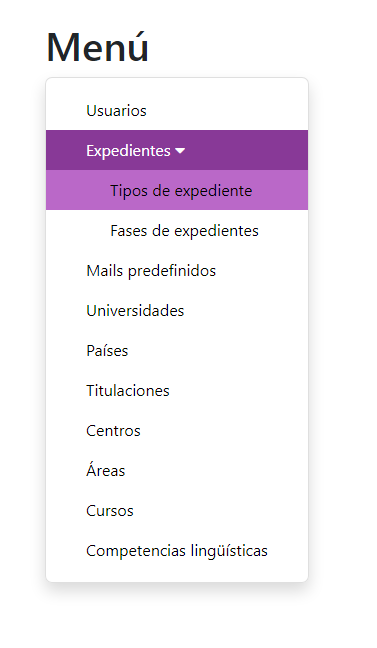
\includegraphics[height=0.4\textheight]{img/Capturas de twinX/sidebar_panel}
	\caption{Menú lateral del panel en twinX}
	\label{fig:sidebarpaneltwinX}
\end{figure}

Para conseguir el funcionamiento de \textit{dropdown}, hemos escrito el siguiente código con jQuery (\texttt{backend/web/js/dropdown\_expediente\_panel.js}):

\begin{minted}[frame=lines,breaklines]{javascript}
	let submenusExpedientes = ['tipo-expediente', 'fase-expediente', 'envio-mail-fase'];
	$(document).ready(function() {
		submenusExpedientes.forEach(function (str) {
			if (window.location.pathname.includes(str))
			toggleCollapse();
		});
	});
\end{minted}

Tras la creación del menú CRUD de los usuarios (el modelo ya está creado con anterioridad con la migración), se crean, por un lado, la clase de controlador, \texttt{UserController.php}, dentro de \texttt{backend/modules/panel/controllers}. Un nivel más arriba, en \texttt{views}, se tiene una nueva carpeta llama \texttt{user}, que posee los siguientes archivos:

\begin{itemize}
	\item \textbf{\texttt{\_form.php}}: es el formulario (\texttt{ActiveForm} de Yii, que renderiza un elemento \texttt{form} de HTML) que es utilizado por las vistas que necesiten cargar el formulario de datos de un usuario en la base de datos.
	\item \textbf{\texttt{create.php}}: es el receptor de la acción \texttt{create} del controlador, el cual renderiza el formulario \texttt{\_form.php} para crear un usuario nuevo.
	\item \textbf{\texttt{update.php}}: también carga el mismo formulario, pero recibe la acción \texttt{update} del controlador, el cual envía la información que ya se tiene sobre un usuario en concreto.
	\item \textbf{\texttt{view.php}}: la vista de los datos del usuario en detalle.
\end{itemize}

Cada uno de estos archivos conforma la vista de un componente; en este caso, el de usuario.

Sobre los controladores, diremos que son los orquestadores de lo que se ve en pantalla, hasta el punto de que, de alguna manera, al escribir en la barra de direcciones \texttt{localhost/panel/user/view?id=3}, lo que ocurre es que se llama al método \texttt{actionView} de la clase \texttt{UserController}. Es decir, se llama al método \texttt{actionX} de la clase \texttt{yController}, donde claramente «x» es \texttt{view} en nuestro caso e «y», \texttt{User}. Con esto, y tras la atenta visualización de la ausencia de un archivo \texttt{delete.php} en la vista, podemos imaginar que al ir a \texttt{localhost/panel/user/delete?\\id=3} se ejecutará el método \texttt{actionDelete}, que al igual que \texttt{actionView} acepta el parámetro \texttt{\$id}. Pensemos, pues, que para eliminar un registro no necesitamos ninguna vista, pero sí un método en el controlador. Al fin y al cabo, ese método ordenará al modelo eliminar el registro, que es lo único que necesitábamos.

Los modelos son clases más sencillas, las cuales tienen la especificación de los atributos que tiene la tabla en concreto en base de datos, los métodos para recuperar los objetos de otros modelos a los que referencian (por ejemplo, como hemos dicho antes, una universidad pertenece a un país y, por tanto, el objeto del modelo de \texttt{Pais} estará dentro de \texttt{Universidad}), y otros métodos que generalmente creemos nosotros para acceder a datos externos de manera más rápida.

Una vez hemos hecho un recorrido por los tres grandes tipos de clases que tenemos --modelos, vistas y controladores--, podemos entonces comprender el significado de nuestro patrón arquitectónico y la influencia que tiene en twinX respecto de lo coherente que resulta el establecer esta separación.

Volviendo al desarrollo, tras crear con Gii la tabla CRUD (figura \ref{fig:giicruduser}), el resultado es el menú de la figura \ref{fig:usuariostwinX}. Normalmente, las tablas CRUD suelen tener un botón verde que permiten crear un nuevo registro, pero en el caso de los usuarios, se ha eliminado, ya que al crearlo manualmente desde este menú, no se genera un hash para la contraseña, al mismo tiempo que tampoco tiene gran relevancia el poder crear usuarios desde el panel de control, cuando el principal interés está puesto en gestionar los permisos de los integrantes de la comunidad.

\begin{figure}
	\centering
	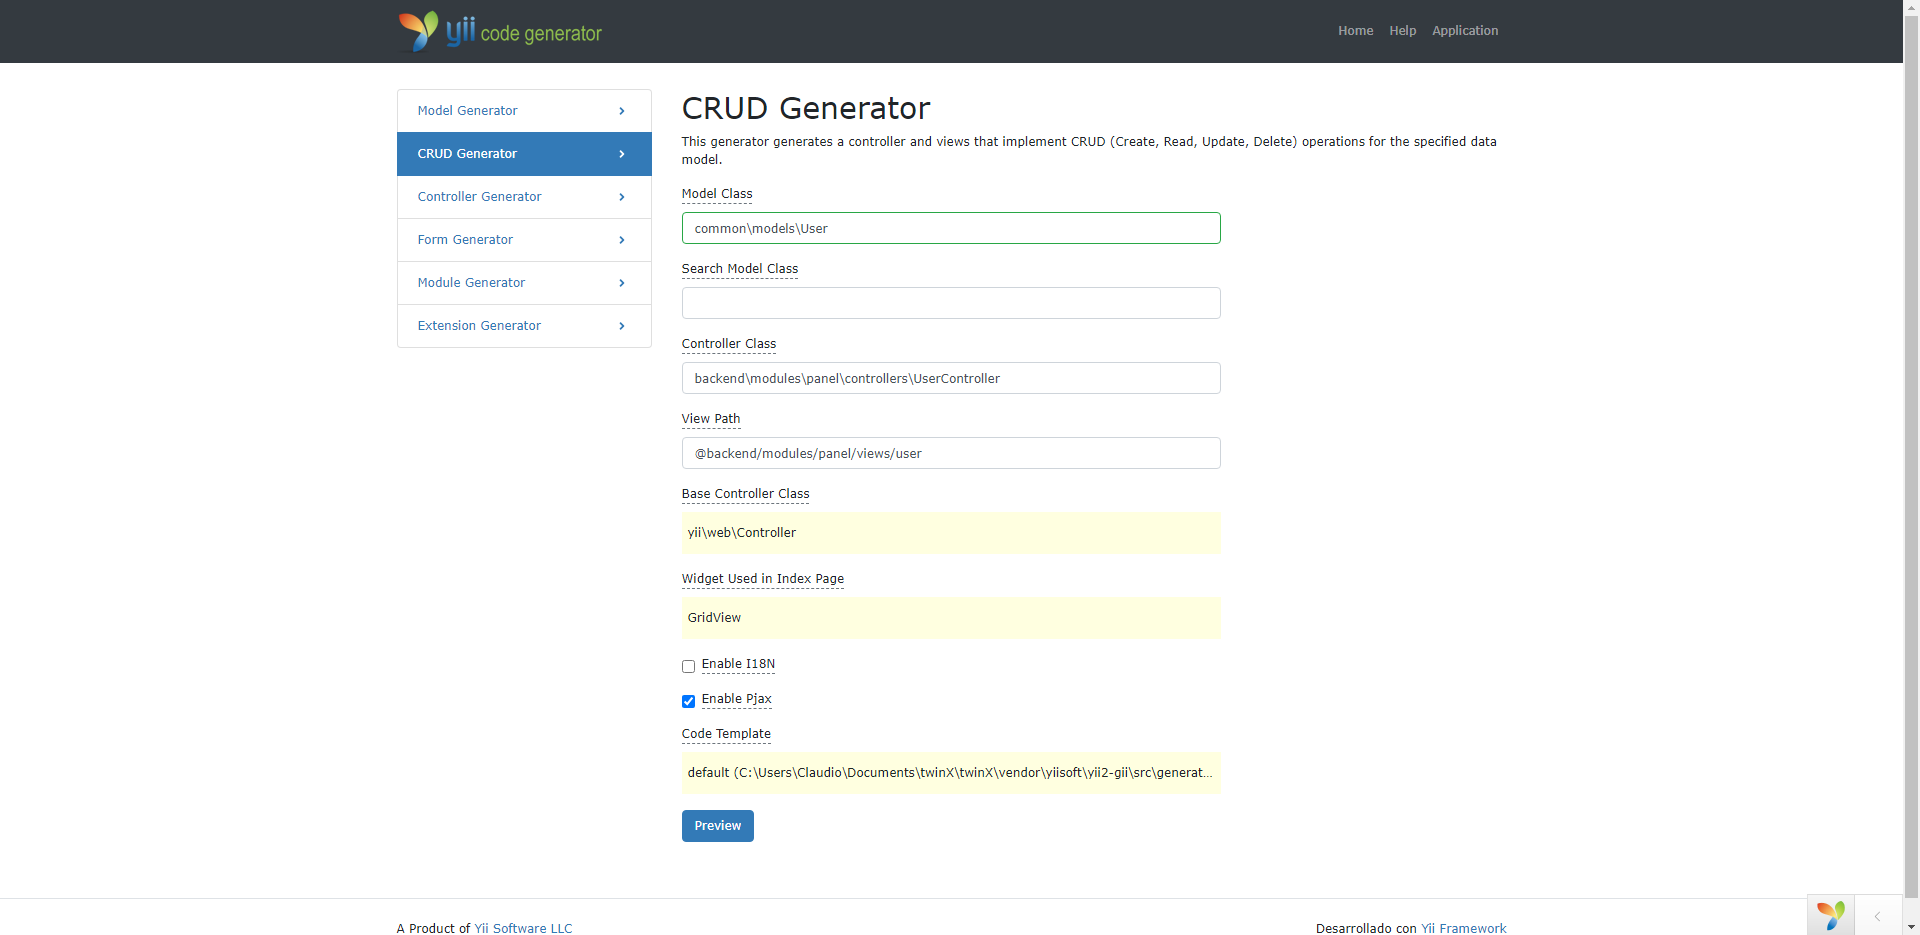
\includegraphics[width=\textwidth]{img/Capturas de twinX/gii_crud_user}
	\caption{Generación de la tabla CRUD de User}
	\label{fig:giicruduser}
\end{figure}


\begin{figure}
	\centering
	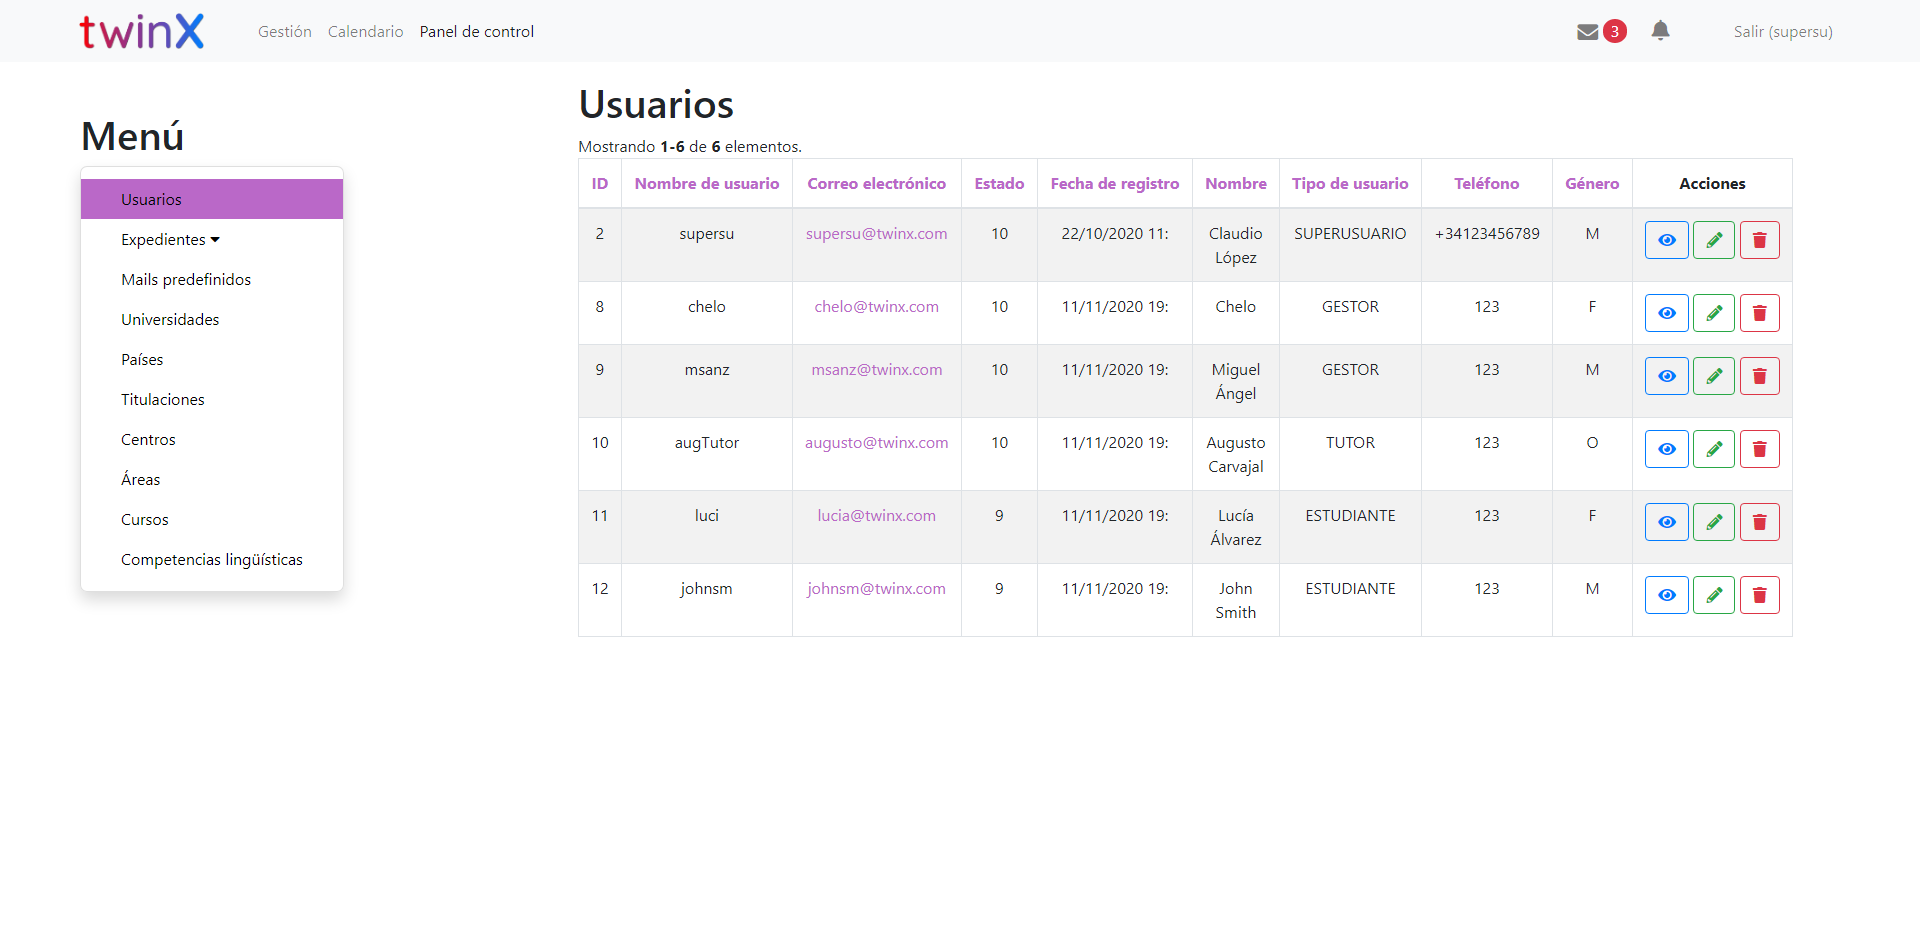
\includegraphics[width=\textwidth]{img/Capturas de twinX/usuarios_twinX}
	\caption{Menú de usuarios en twinX}
	\label{fig:usuariostwinX}
\end{figure}

Como ya hemos señalado con anterioridad, se tomó la decisión de mantener las vistas de los registros almacenados sin apenas modificar en este módulo de panel de control. Por defecto, lo que podemos ver en la interfaz de vista de un registro es lo que encontramos en la figura \ref{fig:vistatitulaciontwinX}.

\begin{figure}
	\centering
	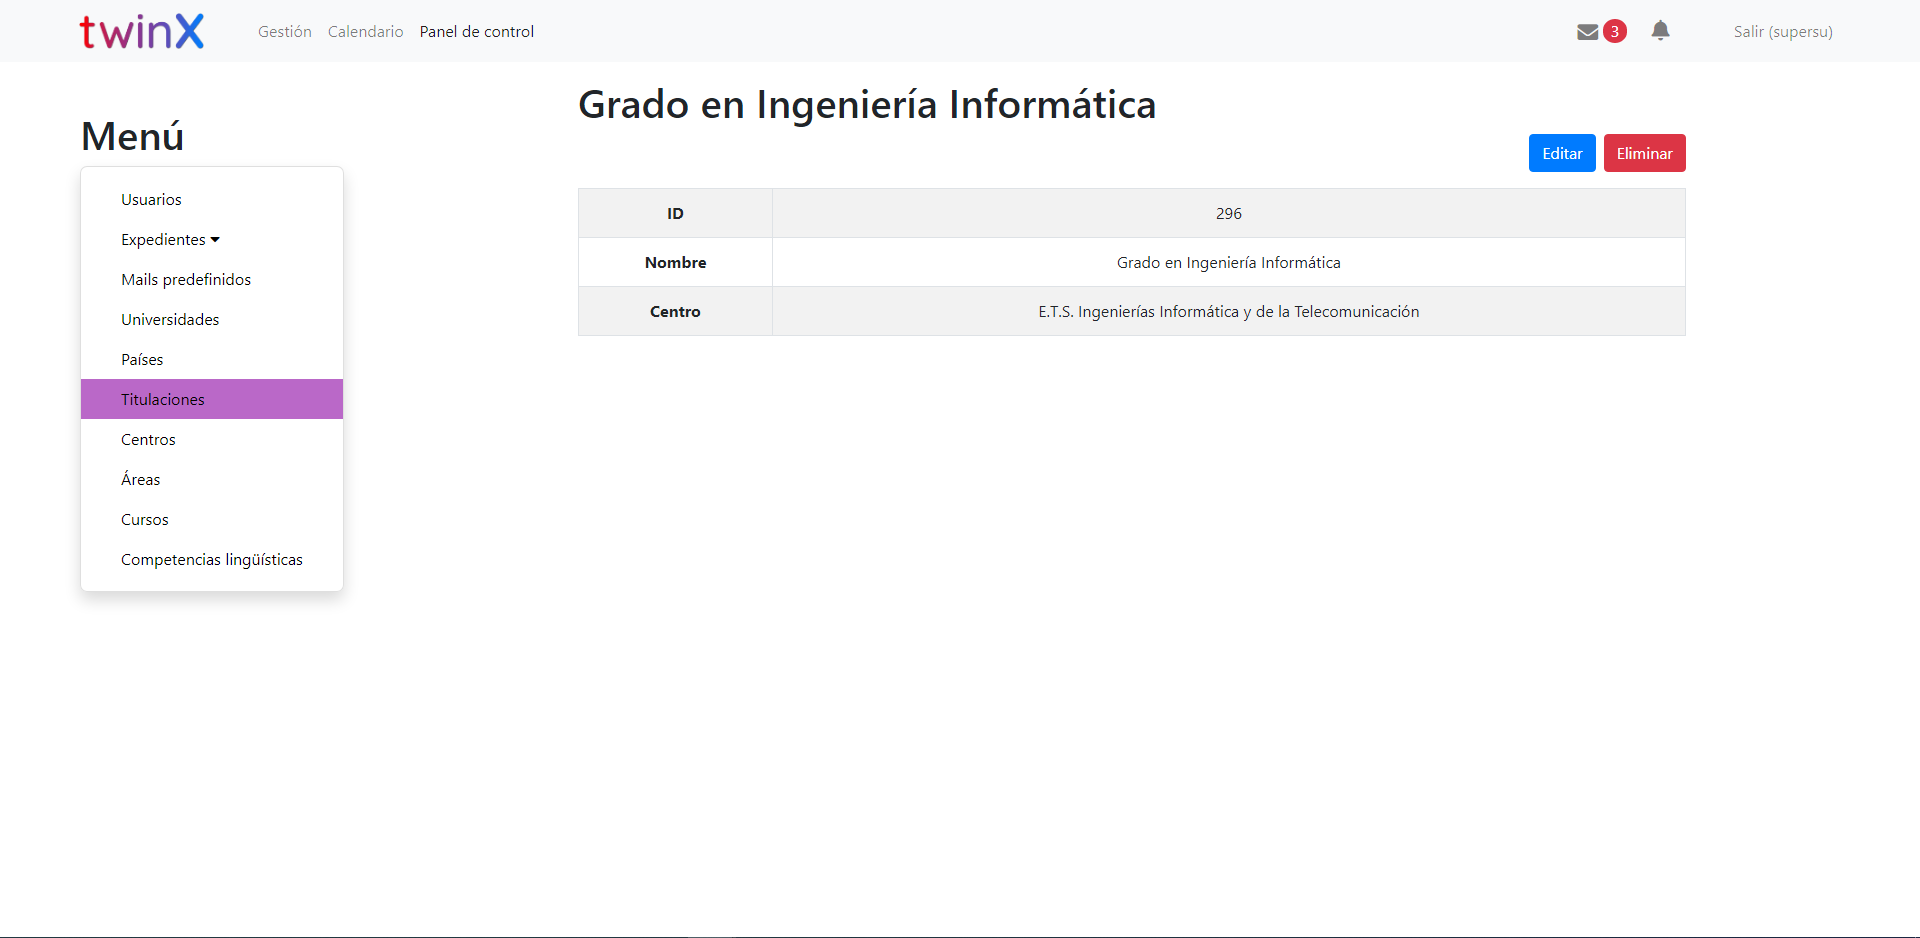
\includegraphics[width=\textwidth]{img/Capturas de twinX/vista_titulacion}
	\caption[Vista de un registro en twinX]{Vista de un registro en twinX (menú de titulaciones)}
	\label{fig:vistatitulaciontwinX}
\end{figure}

Por defecto, Gii pone ciertos botones justo a la izquierda de las cabeceras de las tablas y de las vistas. Sin embargo, hemos tomado la decisión de modificar esto, como se puede apreciar en la figura \ref{fig:vistatitulaciontwinX}, donde los botones de «editar» y «eliminar» están a la derecha. El motivo es porque mayormente en las tablas del menú \texttt{index} de cada categoría, como la de la figura \ref{fig:fasesexpedientesindex} se podía ver un exceso de información de haber dejado el botón en la izquierda, pues tendríamos el título, el indicador del total de elementos de la tabla y el botón. Por tanto, hemos dejado todos los botones a la derecha en las sucesivas vistas de los menús de toda la plataforma.

Por supuesto, no hemos hecho los cambios de forma manual, sino que se ha modificado el código del generador de Gii para que todas las genere automáticamente como describimos. Esto es posible modificando el archivo \texttt{index.php} para la tabla del menú y el \texttt{view.php} para la vista de un registro en el directorio \texttt{vendor/yiisoft/yii2-gii/src/generators/crud/default/views}\footnote{Este directorio no se encuentra en el respositorio de GitHub \cite{repogit}, dado que forma parte de los archivos del motor de Yii y se encuentran dentro del archivo \texttt{.gitignore}, por lo que no se guardan, dado que pueden obtenerse clonando el repositorio de Yii \cite{yii2advanced}}. Sobre el primero de los archivos, diremos que también hemos hecho las pertinentes modificaciones para que cada una de las vistas tenga el botón del ojo (acceso a la vista en detalle) el lápiz (para editar la entrada) y la papelera (para la eliminación) para interaccionar con cada registro en concreto.

\begin{figure}
	\centering
	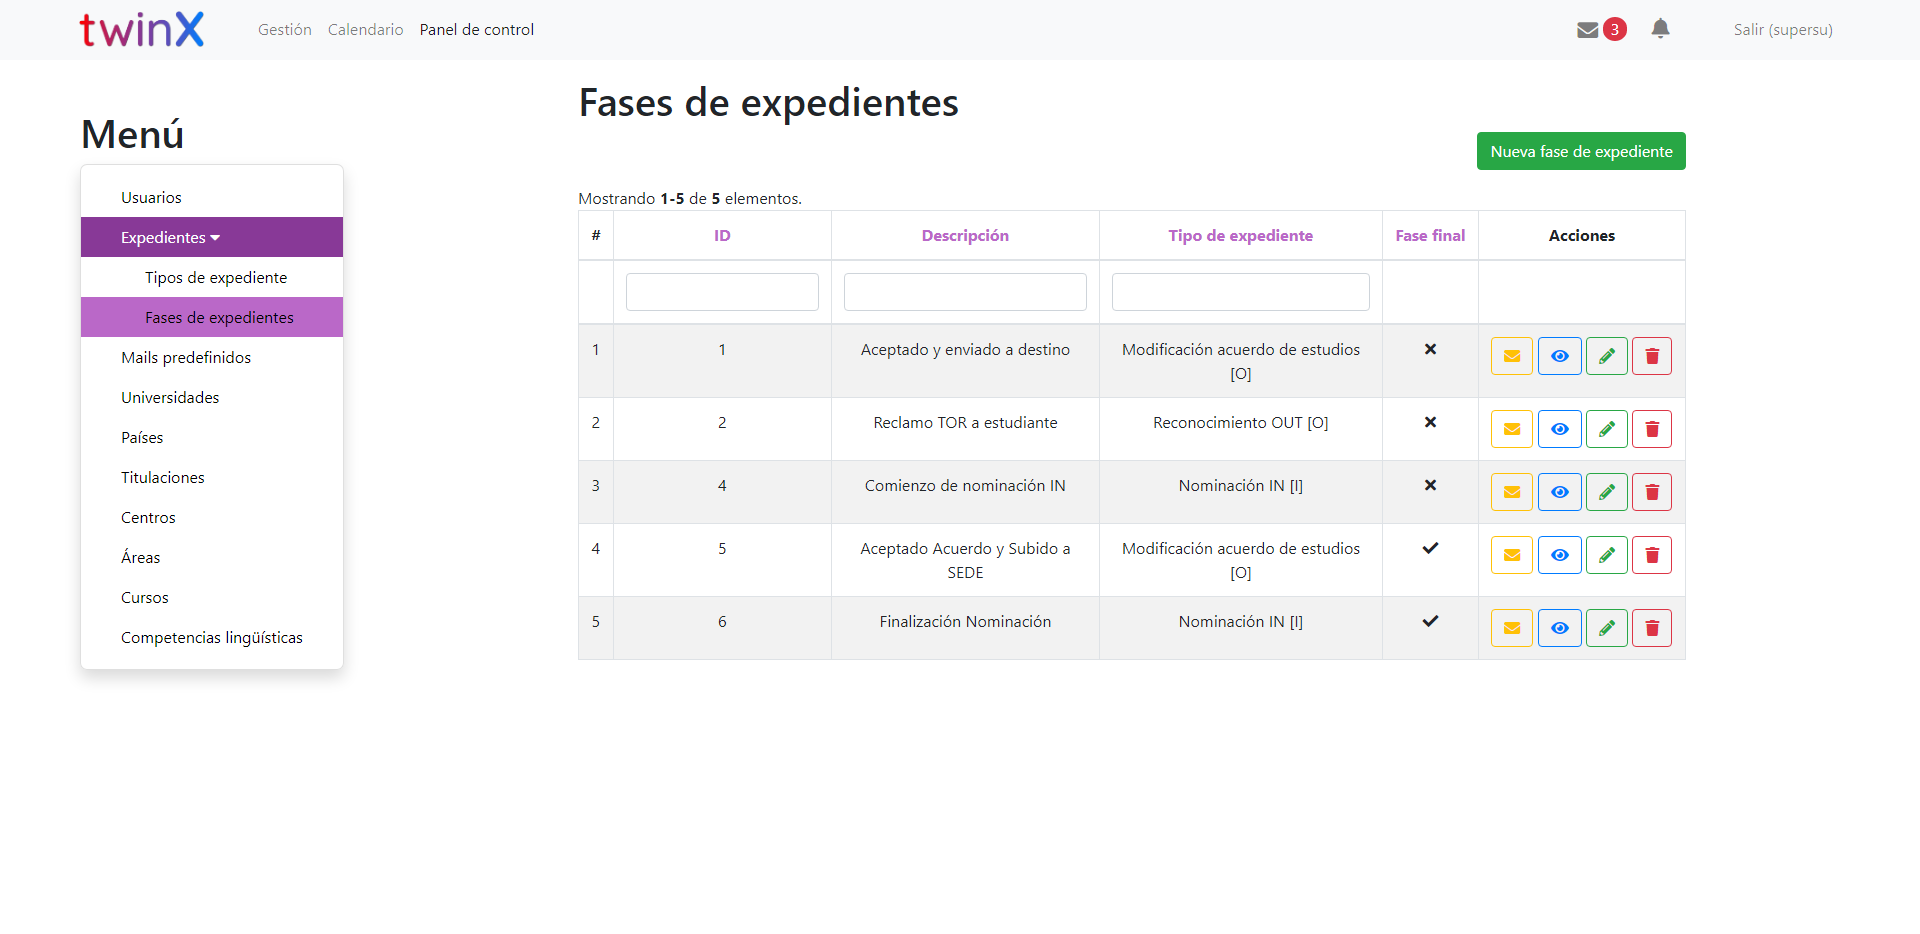
\includegraphics[width=\textwidth]{img/Capturas de twinX/fases_expedientes_index}
	\caption{Menú de fases de expedientes en twinX}
	\label{fig:fasesexpedientesindex}
\end{figure}

Por último, vamos a destacar la vista de una fase de expediente. Recordemos que el procesar una fase implicaba enviar varios correos a responsables y a destinatarios relacionados con la situación del estudiante (o incluso a él mismo). Por tanto, hemos incluido en la vista de las fases, los mensajes que se enviarían tras procesarla (figura \ref{fig:fasesexpedientesvista}). También podemos verlos pulsando en el botón amarillo con el sobre de la figura \ref{fig:fasesexpedientesindex}, donde se dan aún más opciones al usuario. La implementación de esta parte no es compleja pero sí tediosa, por lo que vamos a omitir su explicación por el momento, dado que en la próxima sección veremos otro ejemplo, ya que en el módulo de gestión \ref{sec:gestion} hemos diseñado una vista compuesta de forma similar.

\begin{figure}
	\centering
	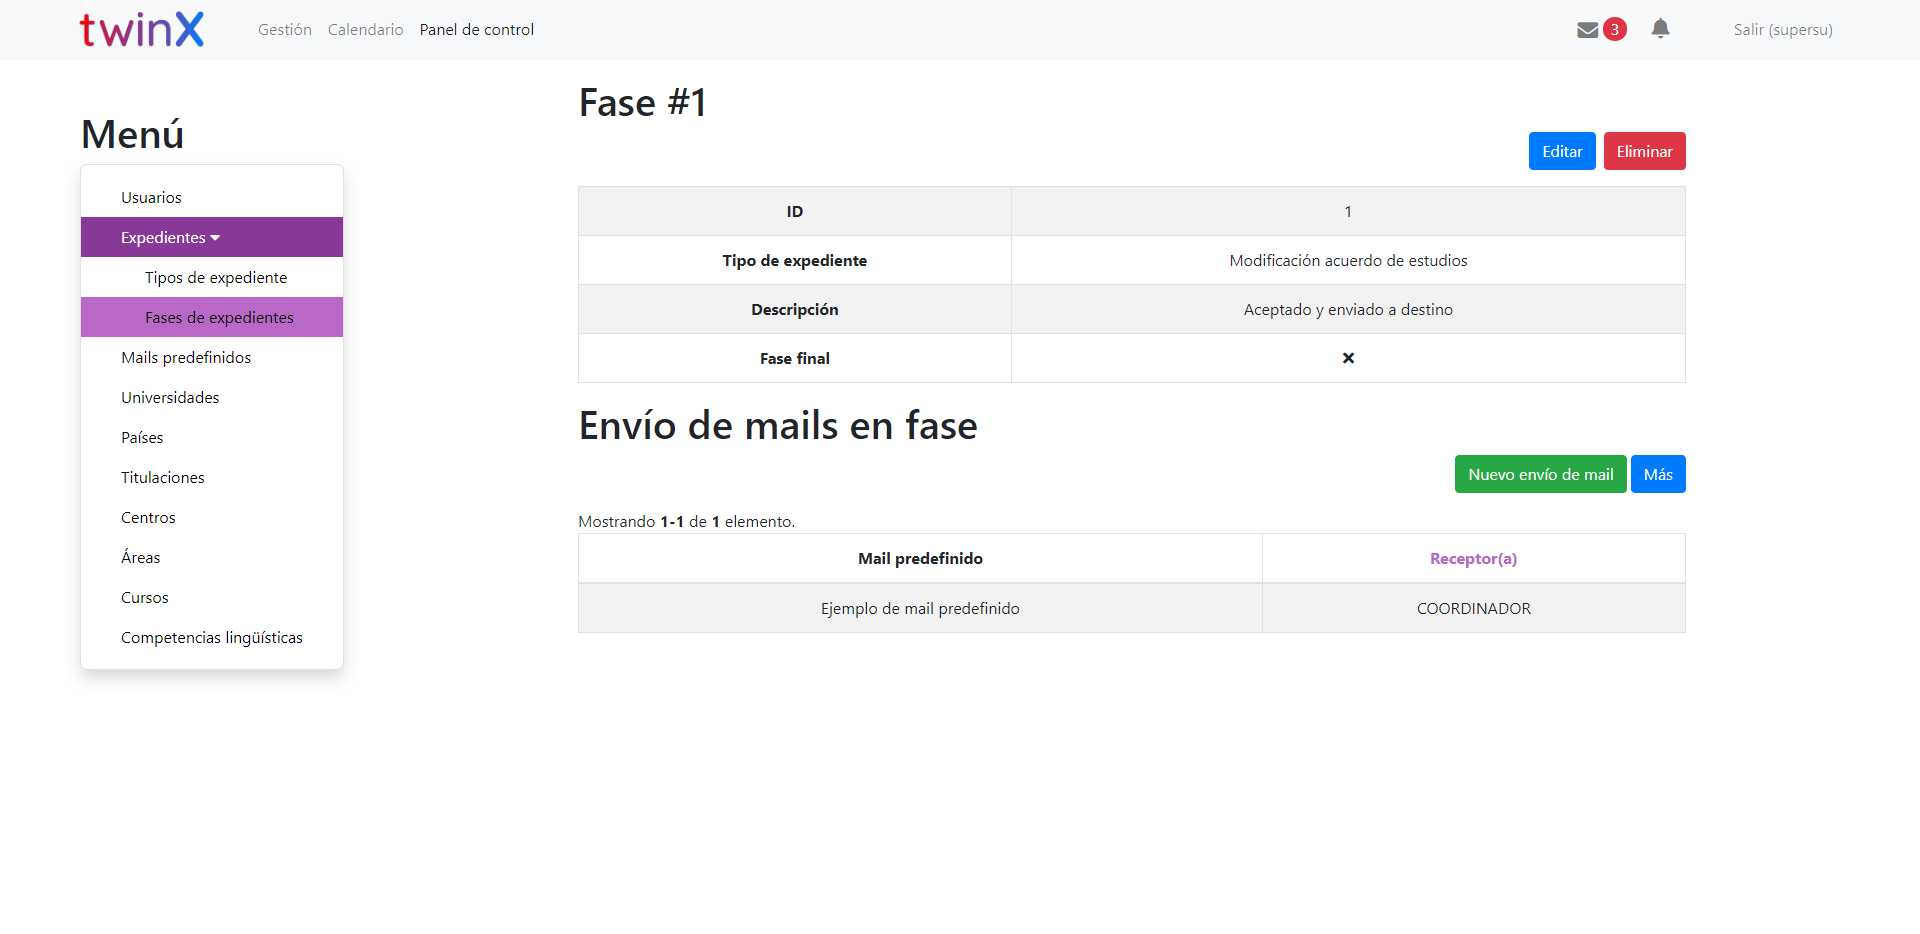
\includegraphics[width=\textwidth]{img/Capturas de twinX/fases_expedientes_vista}
	\caption{Vista de una fase de expediente en twinX}
	\label{fig:fasesexpedientesvista}
\end{figure}



\section{Desarrollo del módulo de gestión}
\label{sec:gestion}

Para desarrollar esta parte de la aplicación, también se ha creado un módulo y las tablas CRUD pertinentes para cada una de las secciones de Gestión. Recordamos que es el corazón de la aplicación, donde los gestores acudirían diariamente a desempeñar su trabajo: consulta de la información referente a un estudiante, tramitación de algún expediente, cambios en su acuerdo de estudios, etc.

\subsection{Integración del menú de convenios}

Uno de los mayores desafíos ha sido, como era de imaginar a la hora de ver el modelo de la base de datos (figura \ref{fig:modeloBD}), el diseñar un formulario para los convenios recogido y no puesto tal cual sale de Gii. Para ello, hemos empleado el objeto de Bootstrap \texttt{card} y \texttt{accordion}. Conforme vamos desplegando cada una de las secciones, las otras se cierran para no ocupar espacio en la pantalla y hacer que el usuario se centre en la introducción de los datos en una sección concreta. También hemos usado tarjetas a distintos niveles para estructurar los formularios de la mejor manera posible (figuras \ref{fig:creacionconvenio1} y \ref{fig:creacionconvenio2})

\begin{figure}
	\centering
	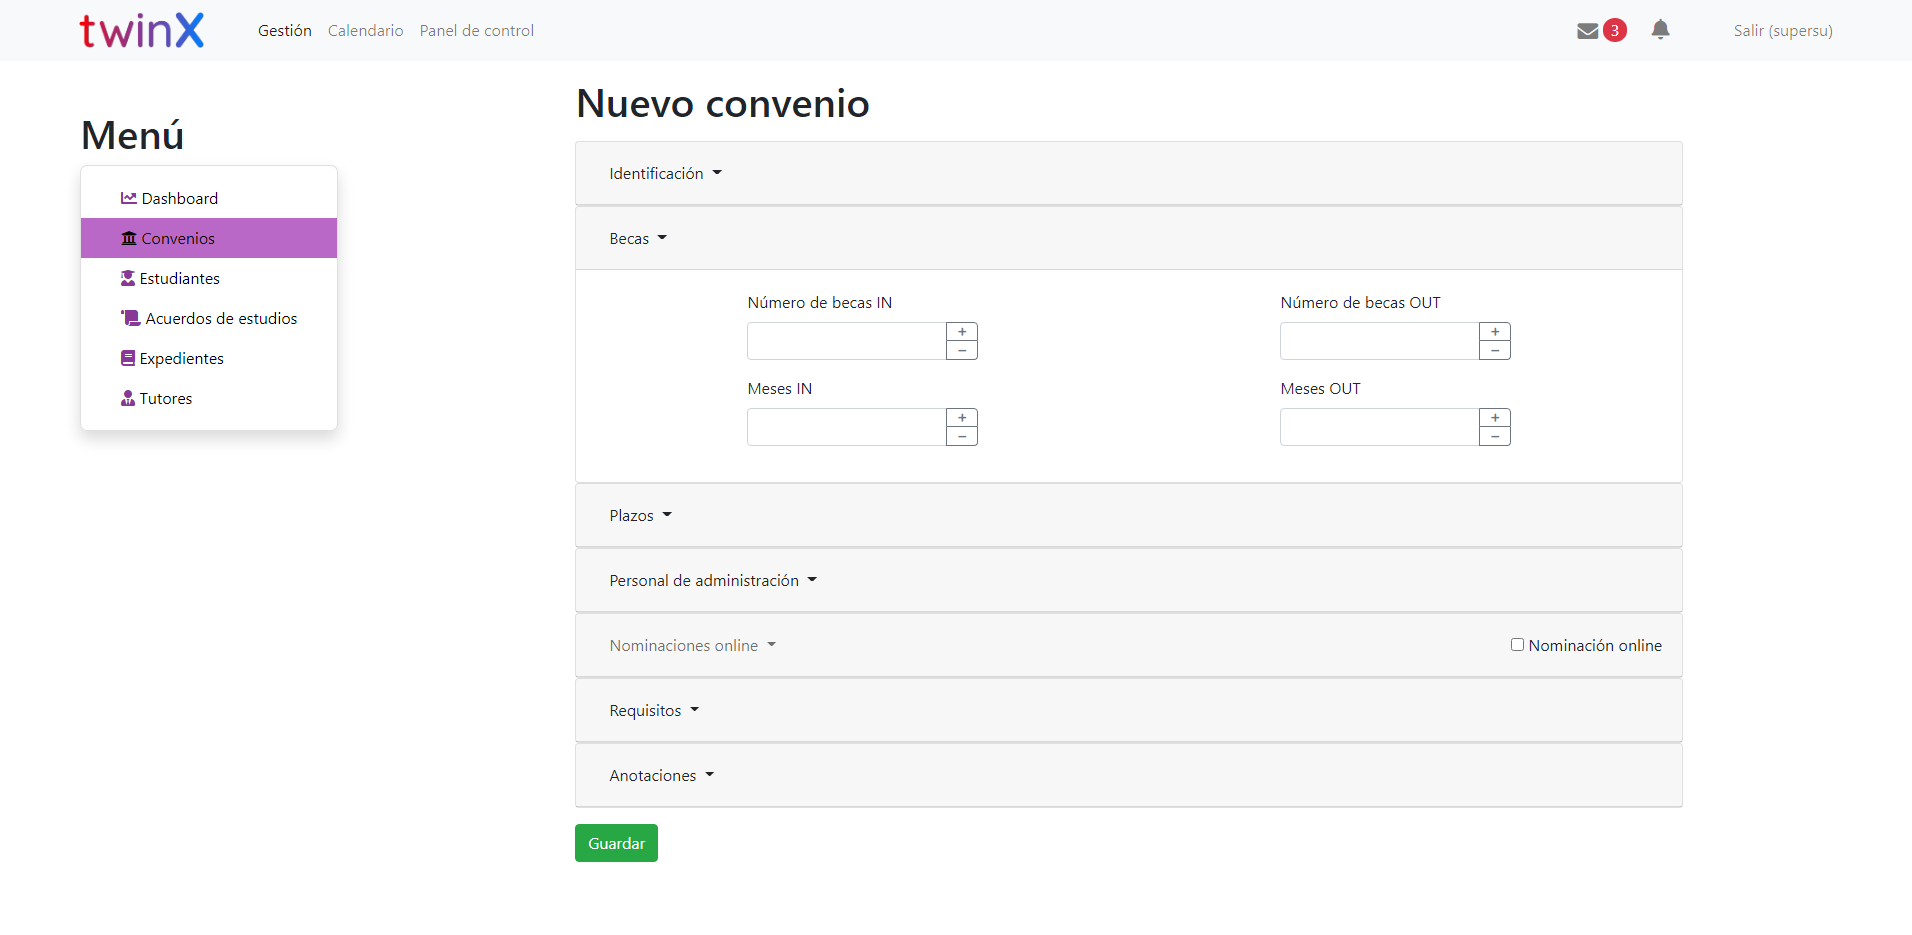
\includegraphics[width=\textwidth]{img/Capturas de twinX/creacion_convenio_1}
	\caption{Creación de un convenio en twinX}
	\label{fig:creacionconvenio1}
\end{figure}

\begin{figure}
	\centering
	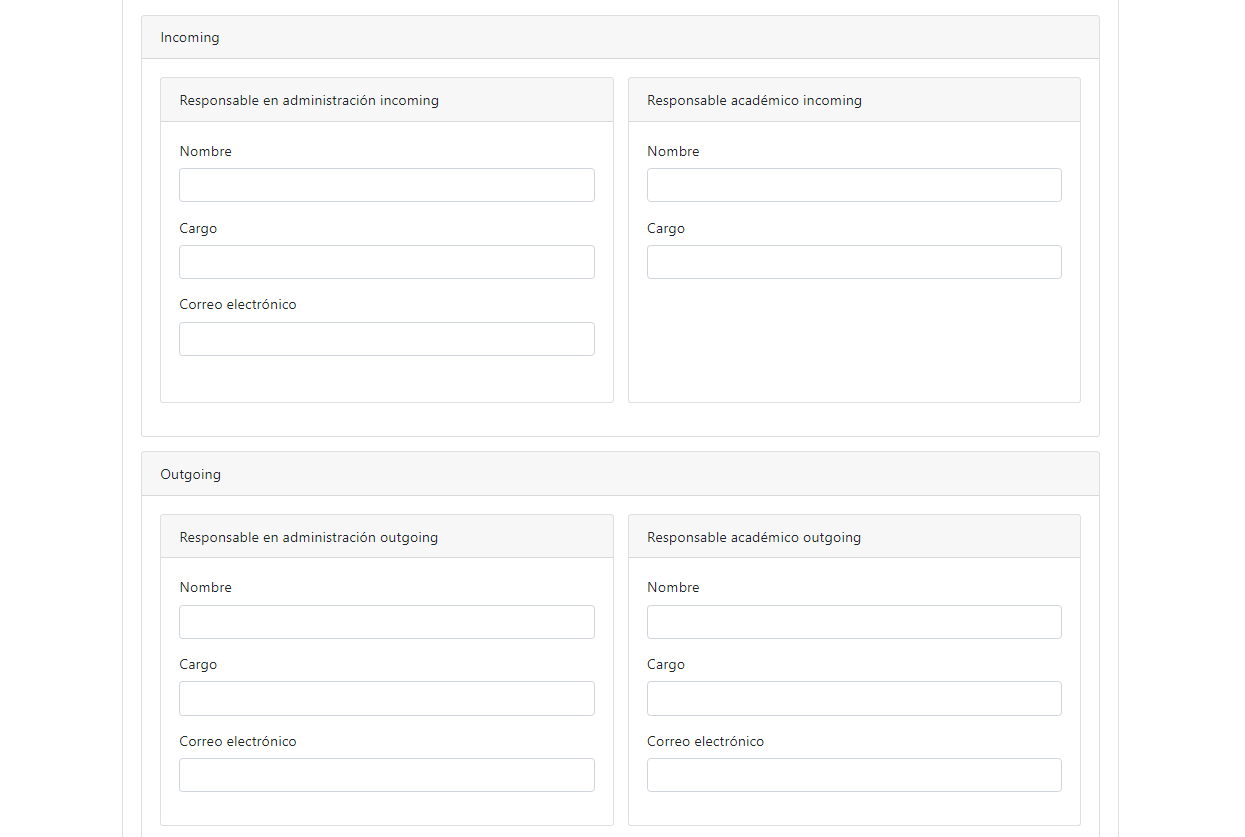
\includegraphics[width=\textwidth]{img/Capturas de twinX/creacion_convenio_2}
	\caption[Creación de un convenio en twinX 2]{Creación de un convenio en twinX: introducción de datos de los responsables externos}
	\label{fig:creacionconvenio2}
\end{figure}

Por defecto, Gii espera que en campos donde en la tabla se tiene una restricción de clave externa se introduzca, mediante un campo de texto libre, un identificador, por ejemplo, del país del convenio. Sin embargo, este es une de los numerosos cambios que se comienzan haciendo al recibir el código generado: adaptarlo al usuario. Para ello y durante todo el proyecto en general, hemos hecho uso de librerías del autor \textit{Kartik} \cite{krajee} y como resultado, tenemos elementos que ya están disponibles en Yii2 como es la inserción de un menú \textit{dropdown} para escoger entre varias opciones, pero potenciado con una búsqueda, por ejemplo, como se aprecia en la figura \ref{fig:creacionconvenio3}. Pensemos que elementos como este son indispensables, pues en el uso cotidiano, twinX almacenaría cientos de estudiantes, decenas de universidades y convenios tal y como hace TWINS hasta el momento; por tanto, la opción de un desplegable estático no funcionaría en este contexto. Su uso es verdaderamente sencillo, una vez que nos familiarizamos con la sintaxis:

\begin{minted}[frame=lines]{php}
	<?php
	(...)	
	 <?= $form->field($model, 'cod_pais')->widget(Select2::className(), [
		'data' => ArrayHelper::map(Pais::find()->all(), 'iso', 'nombreISO'),
		'theme' => Select2::THEME_KRAJEE_BS4,
		'options' => [
			'placeholder' => 'Seleccione un país',
		]
	]) ?>
	
\end{minted}


\begin{figure}
	\centering
	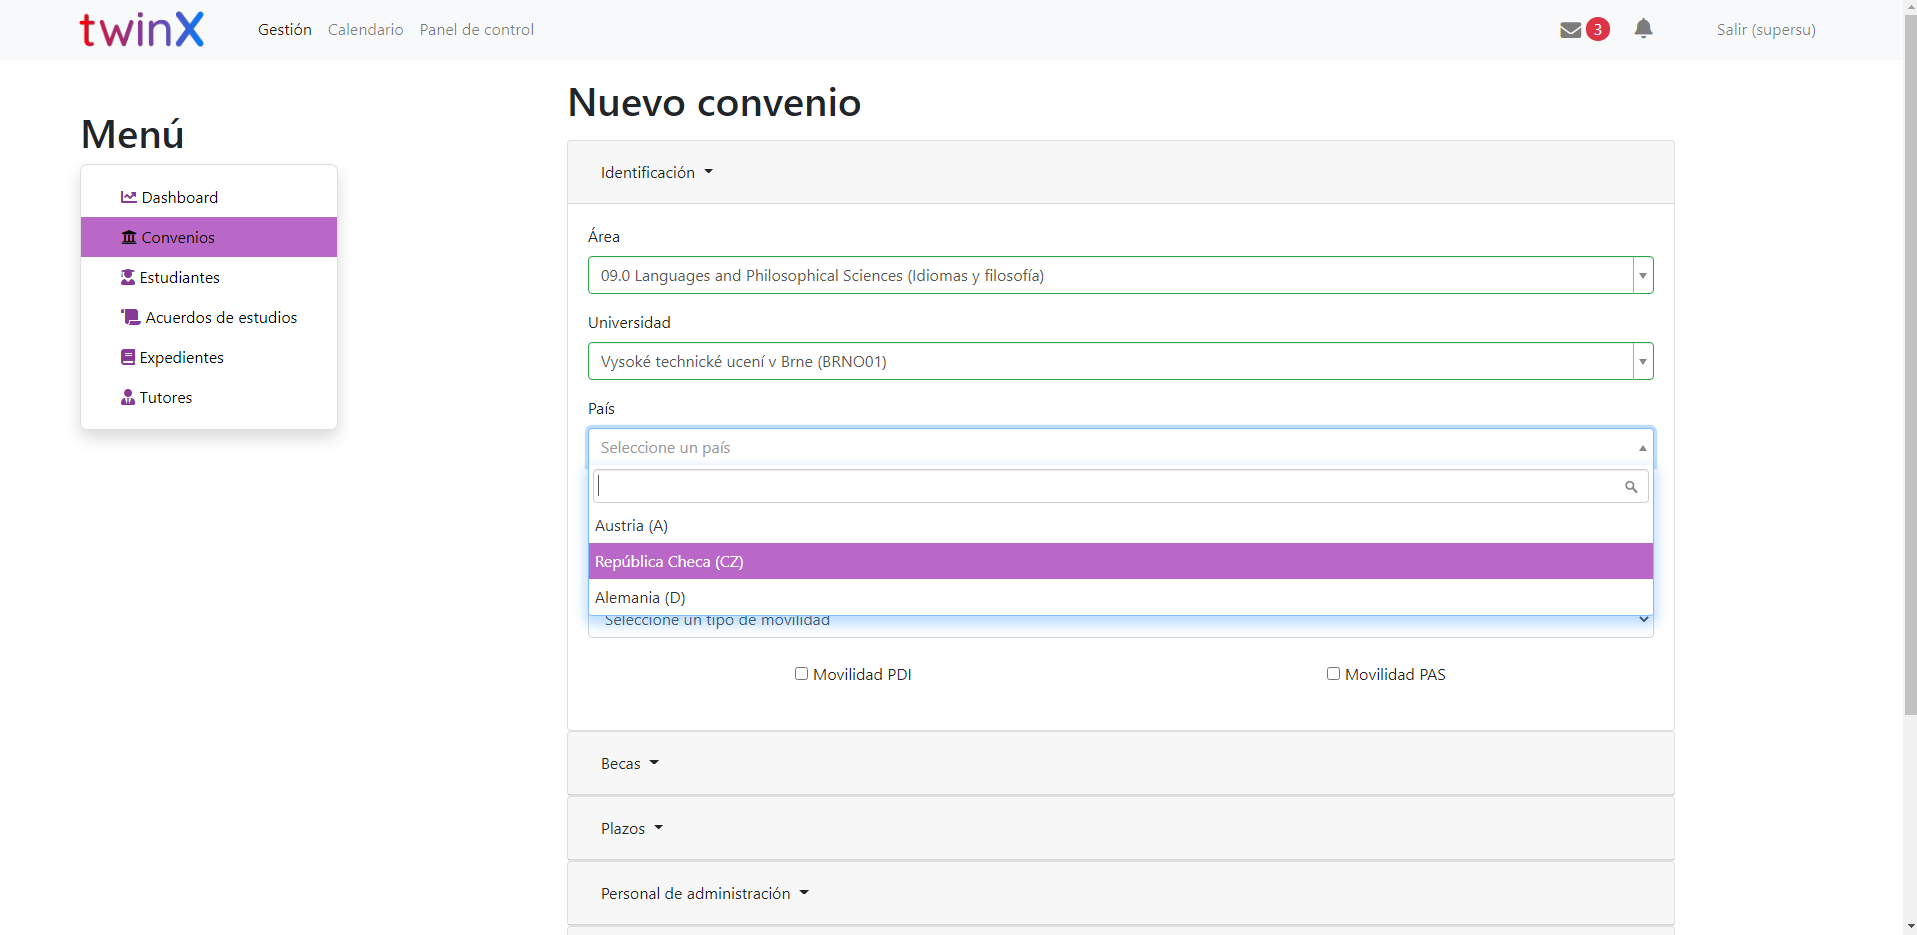
\includegraphics[width=\linewidth]{img/Capturas de twinX/creacion_convenio_3}
	\caption[Creación de un convenio en twinX 3]{Creación de un convenio en twinX: introducción de datos externos al modelo \texttt{Convenio}}
	\label{fig:creacionconvenio3}
\end{figure}

Otra dificultad de la implementación del formulario de los convenios estaba en la selección de los requisitos lingüísticos. Éstos se almacenan en una tabla aparte, pero existe una relación muchos a muchos que relaciona un convenio con varias competencias o la pertenencia de una sola competencia a muchos convenios. El problema estaba cuando queríamos asociar un par \texttt{(id\_convenio, id\_requisito)} sin tener de antemano la ID del convenio que se está creando. Para ello ha sido necesario crear una \textbf{transacción}. Es decir, primeramente tenemos que asegurarnos de que guardamos todos los datos del convenio. Acto seguido, asociar los requisitos lingüísticos que se han escogido para el convenio a crear y, después, guardar los cambios. Si alguna de estas acciones no prospera, tendremos que cancelar todo y devolver la tabla a su estado anterior. Esto podemos conseguirlo sobrecargando el método de guardado, \texttt{save}.

Es más, también hemos de tener en cuenta que el tratamiento de los requisitos puede darse en la edición del convenio, con lo cual, puede haber requisitos ya en la tabla que tenemos que recuperar, y a la hora de ejecutar la transacción, evaluar cuáles estaban ya en la tabla de la relación convenio - requisito y dejarlos intactos, cuáles han de ser eliminados y cuáles insertados como nuevos registros.

Para ello, tenemos que crear una nueva clase \texttt{ConvenioForm} que extienda a \texttt{Convenio} (modelo) y herede sus métodos. Entonces, programamos toda esta funcionalidad que hemos descrito y solo cuando sea necesario, hacemos la llamada a este nuevo modelo. Una de las características más novedosas es la sobrecarga del método \texttt{afterFind}, que ejecuta justo después de buscar la recuperación de los requisitos actuales del convenio (si los tiene). Gracias a ello, podemos trabajar con un array de requisitos y ejecutar las acciones descritas:

\begin{minted}[frame=lines, breaklines]{php}
<?php
(...)

class ConvenioForm extends Convenio
{
	public $requisitos = [];
	private $_requisitos;
	
	public function save($runValidation = true, $attributeNames = null)
	{
		$transaction = \Yii::$app->db->beginTransaction();
		
		try {
			if (!parent::save($runValidation, $attributeNames)) {
				return false;
			}
			
			$this->addNewRequisitos();
			$this->deleteOldRequisitos();
			
			$transaction->commit();
			
		}
		
		catch (Exception $e) {
			$transaction->rollBack();
			
			throw $e;
		}
		
		return true;
	}
	
	protected function addNewRequisitos()
	{
		$nuevos = [];
		
		if ($this->isNewRecord) {
			$nuevos = $this->requisitos;
		}
		else if(!empty($this->requisitos)){
			foreach ($this->requisitos as $requisito) {
				if (!in_array($requisito, $this->_requisitos)) {
					$nuevos[] = $requisito;
				}
			}
		}
		
		if(!empty($nuevos)) {
			foreach ($nuevos as $requisito) {
				$relacion = new ReqLingConv();
				
				$relacion->id_conv = $this->id;
				$relacion->id_comp = $requisito;
				
				if (!$relacion->save()) {
					throw new Exception('Error al guardar el requisito');
				}
			}
		}
	}
	
	protected function deleteOldRequisitos()
	{
		foreach ($this->reqLingConvs as $requisito) {
			if (!in_array($requisito->id, $this->requisitos) && $requisito->delete() === false) {
				throw new Exception('Error al guardar los registros');
			}
		}
	}
	
	public function afterFind()
	{
		foreach ($this->reqLingConvs as $requisito) {
			$this->requisitos[] = $requisito->id;
		}
		
		$this->_requisitos = $this->requisitos;
		
		parent::afterFind();
		
	}
}
\end{minted}

El proceso llevado a cabo en \texttt{EstudianteForm} es muy similar, dado que también necesitamos, en el formulario de un estudiante, especificar las competencias lingüísticas que posee.

En el menú de convenios (figura \ref{fig:menuconveniotwinX}) hemos tenido que cambiar bastantes cosas. Para ello, ha sido necesario crear bastantes métodos en el modelo de Convenio. Por ejemplo, para obtener el ratio de estudiantes nominados del total de estudiantes que contiene el convenio. O los convenios con su código completo (código ISO del país, código de la universidad y área de conocimiento según el ISCED\footnote{International Standard Classification of Education}). Del mismo modo, hemos tenido que ajustar la visualización de los nombres de la universidad o del área completos, ya que la generación de código automática solo mostraba los ID en la base de datos:

\begin{minted}[frame=lines]{php}
<?php
(...)
<?= GridView::widget([
	'dataProvider' => $dataProvider,
	'filterModel' => $searchModel,
	'columns' => [
	
		[
			'attribute' => 'numAcuerdos',
			'label' => 'Nº de acuerdos'
		],
		[
			'attribute' => 'nominadosAcuerdos',
			'label' => 'Nominados totales',
			'format' => 'raw'
		],
		[
			'attribute' => 'codConvenio',
			'label' => 'Convenio',
			'format' => 'raw',
		],
		[
			'attribute' => 'nombreCodUni',
			'label' => 'Universidad'
		],
		[
			'attribute' => 'areaCompleta',
			'label' => 'Nombre de la área'
		],
	
	
		'tipo_movilidad',
	
		[
		'class' => 'yii\grid\ActionColumn',
			'template' => '{view}',
			'header' => 'Acciones'
		],
	],
]); ?>
\end{minted}

\begin{figure}
	\centering
	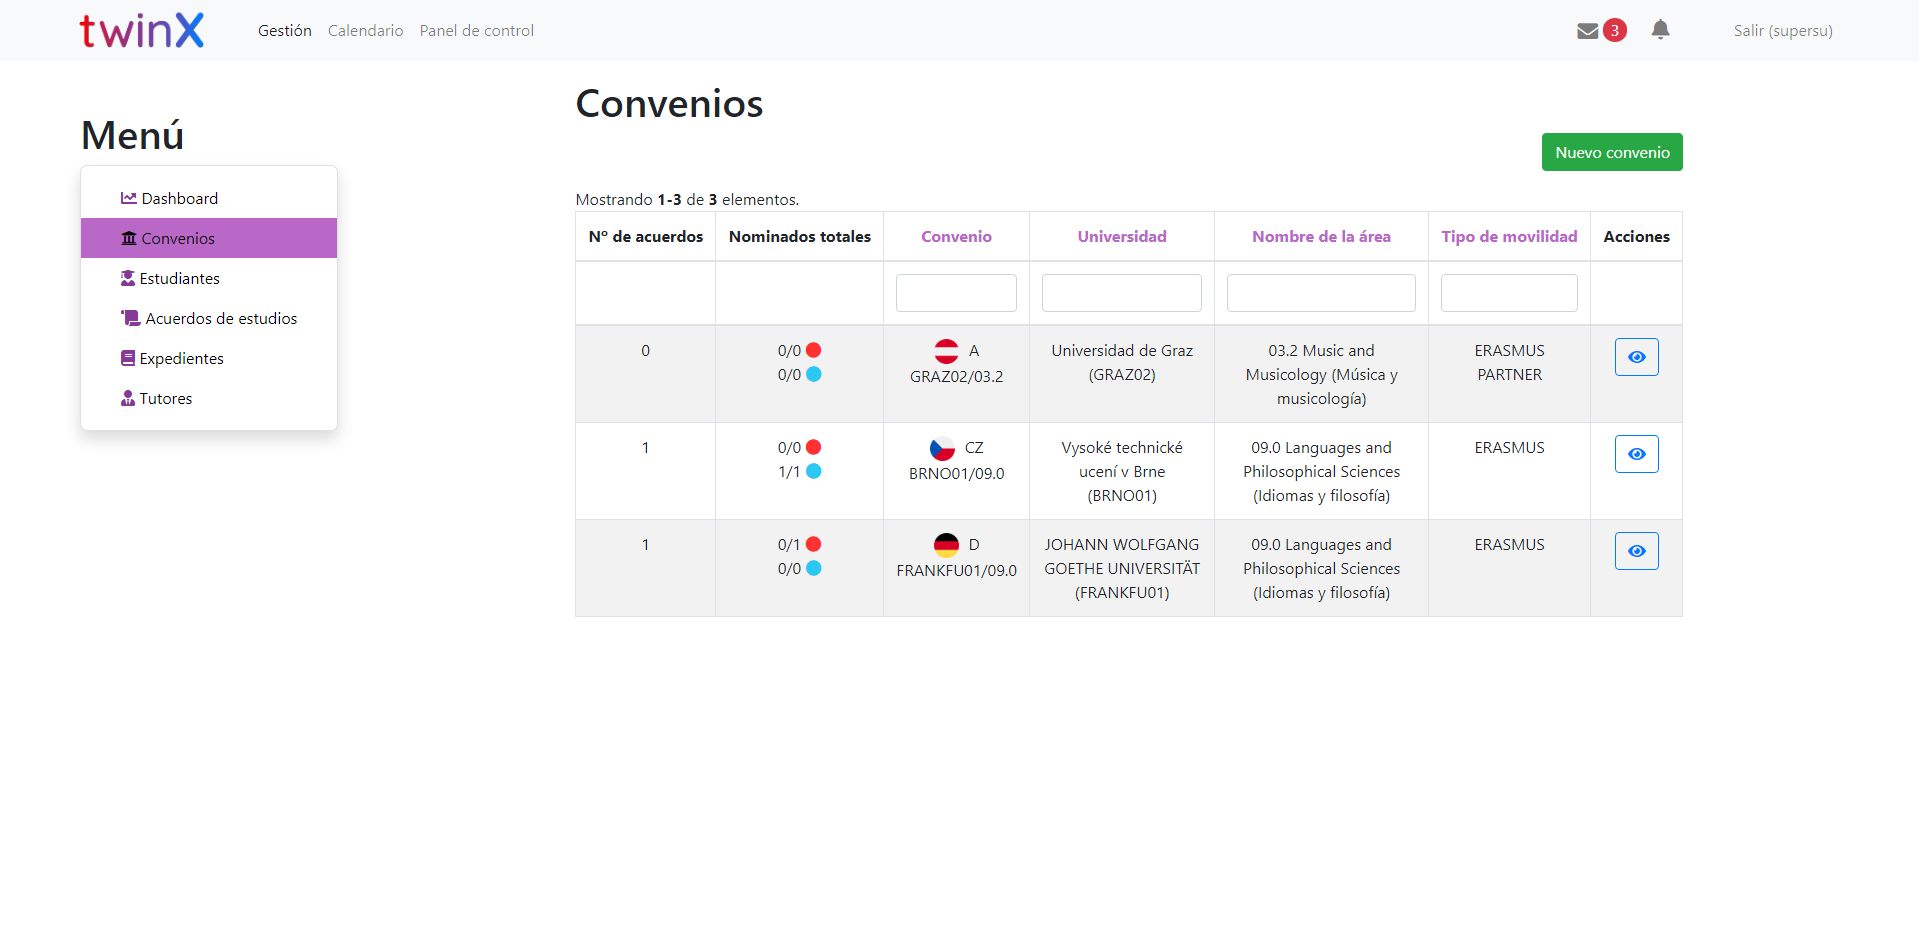
\includegraphics[width=\linewidth]{img/Capturas de twinX/menu_convenio}
	\caption{Menú de convenios en twinX}
	\label{fig:menuconveniotwinX}
\end{figure}

Todos los atributos que vemos en el código son generados por métodos creados en el modelo:

\begin{minted}[frame=lines]{php}
<?php
(...)
public function getNombreCodUni()
{
	return $this->codUni->getNombreCodigo();
}

public function getAreaCompleta()
{
	return $this->codArea->getAreaCompleta();
}
\end{minted}

También podríamos haber hecho ese acceso desde la vista, pero aunque no es una buena práctica, nos complicaría mucho las cosas. El tener los atributos definidos en el modelo, nos permite acceder a ellos desde una clase especial de la que aún no hemos hablado. Son las clases de búsqueda, y se encuentran en \texttt{common/models/search}, nombradas como \texttt{ConvenioSearch} en caso del convenio. Es ahí donde tenemos que decir qué atributos propios hemos definido en nuestro modelo, para poder unir las tablas a las que refieren y así poder hacer tanto búsquedas como ordenaciones, introduciendo términos en los campos de texto de debajo de la cabecera de la tabla y haciendo click en los nombres de los atributos respectivamente. Para conseguir este comportamiento, ha sido necesario hacer en primer lugar, los atributos seguros (\textit{safe}):

\begin{minted}[frame=lines]{php}
<?php
(...)
class ConvenioSearch extends Convenio
{
	public $codConvenio, $nombreCodUni, $areaCompleta;
	
	/**
	* {@inheritdoc}
	*/
	public function rules()
	{
		return [
		(...)
		[['codConvenio', 'nombreCodUni', 'areaCompleta'], 'safe'],
		];
	}
	
	(...)
}
\end{minted}

Después, hacer la unión de la tabla con las demás y configurar las ordenaciones:

\begin{minted}[frame=lines]{php}
<?php
(...)
public function search($params)
{
	$query = Convenio::find();
	
	///
	$query->joinWith(['codPais', 'codArea', 'codUni']);
	
	// add conditions that should always apply here
	
	$dataProvider = new ActiveDataProvider([
	'query' => $query,
	]);
	
	///
	$dataProvider->sort->attributes['codConvenio'] = [
	'asc' => ['pais.iso' => SORT_ASC],
	'desc' => ['pais.iso' => SORT_DESC],
	'default' => SORT_DESC
	];
	
	$dataProvider->sort->attributes['nombreCodUni'] = [
	'asc' => ['universidad.nombre' => SORT_ASC],
	'desc' => ['universidad.nombre' => SORT_DESC],
	'default' => SORT_DESC
	];
	
	$dataProvider->sort->attributes['areaCompleta'] = [
	'asc' => ['area.cod_isced' => SORT_ASC],
	'desc' => ['area.cod_isced' => SORT_DESC],
	'default' => SORT_DESC
	];

	(...)
}

(...)

?>
\end{minted}

Y por último, añadir el filtrado a las búsquedas que se hagan introduciendo texto:

\begin{minted}[frame=lines]{php}
<?php
(...)

->andFilterWhere(['like', 'pais.iso', $this->codConvenio])
->orFilterWhere(['like', 'area.cod_isced', $this->codConvenio])
->orFilterWhere(['like', 'universidad.cod_uni', $this->codConvenio])
->andFilterWhere(['like', 'universidad.nombre', $this->nombreCodUni])
->orFilterWhere(['like', 'universidad.cod_uni', $this->nombreCodUni])
->andFilterWhere(['like', 'area.cod_isced', $this->areaCompleta])
->orFilterWhere(['like', 'area.nombre_isced', $this->areaCompleta])
->orFilterWhere(['like', 'area.nombre_area', $this->areaCompleta]);

(...)

?>
\end{minted}

Esto es extensible a todas las clases donde hemos usado atributos modificados y Yii no conoce la manera de aplicar los filtros, por lo que es obligatorio hacerlo cuando queremos ofrecer otra manera de comunicar una información distinta a la que ofrece el framework por defecto. En muchos casos esto se complica bastante. Por ejemplo, en la unión de las tablas:

\begin{minted}[frame=lines,breaklines]{php}
<?php
(...)

$query->joinWith(['ae.estudiante.usuario', 'ae.estudiante.convenio.codPais', 'tipoExp', 'relExpFases.fase', 'ae.estudiante.convenio.codArea']);

?>
\end{minted}

Este es el código de la clase \texttt{ExpedienteSearch.php}, dadas las numerosas referencias a otras clases externas a ella.

Una vez comentadas las vistas de creación, actualización y de menú principal de los convenios, vamos a abordar la de su vista (figura \ref{fig:vistaconveniotwinX}). Los datos se han separado en distintas secciones de nuevo, pero sin el comportamiento de acordeón que impedía abrir más de una sección al mismo tiempo. Para la vista se debe dar más libertad al usuario, y siempre puede contraer las secciones a su gusto; en cambio, para el formulario, es más importante centrar su atención en una parte de los datos en concreto.

\begin{figure}
	\centering
	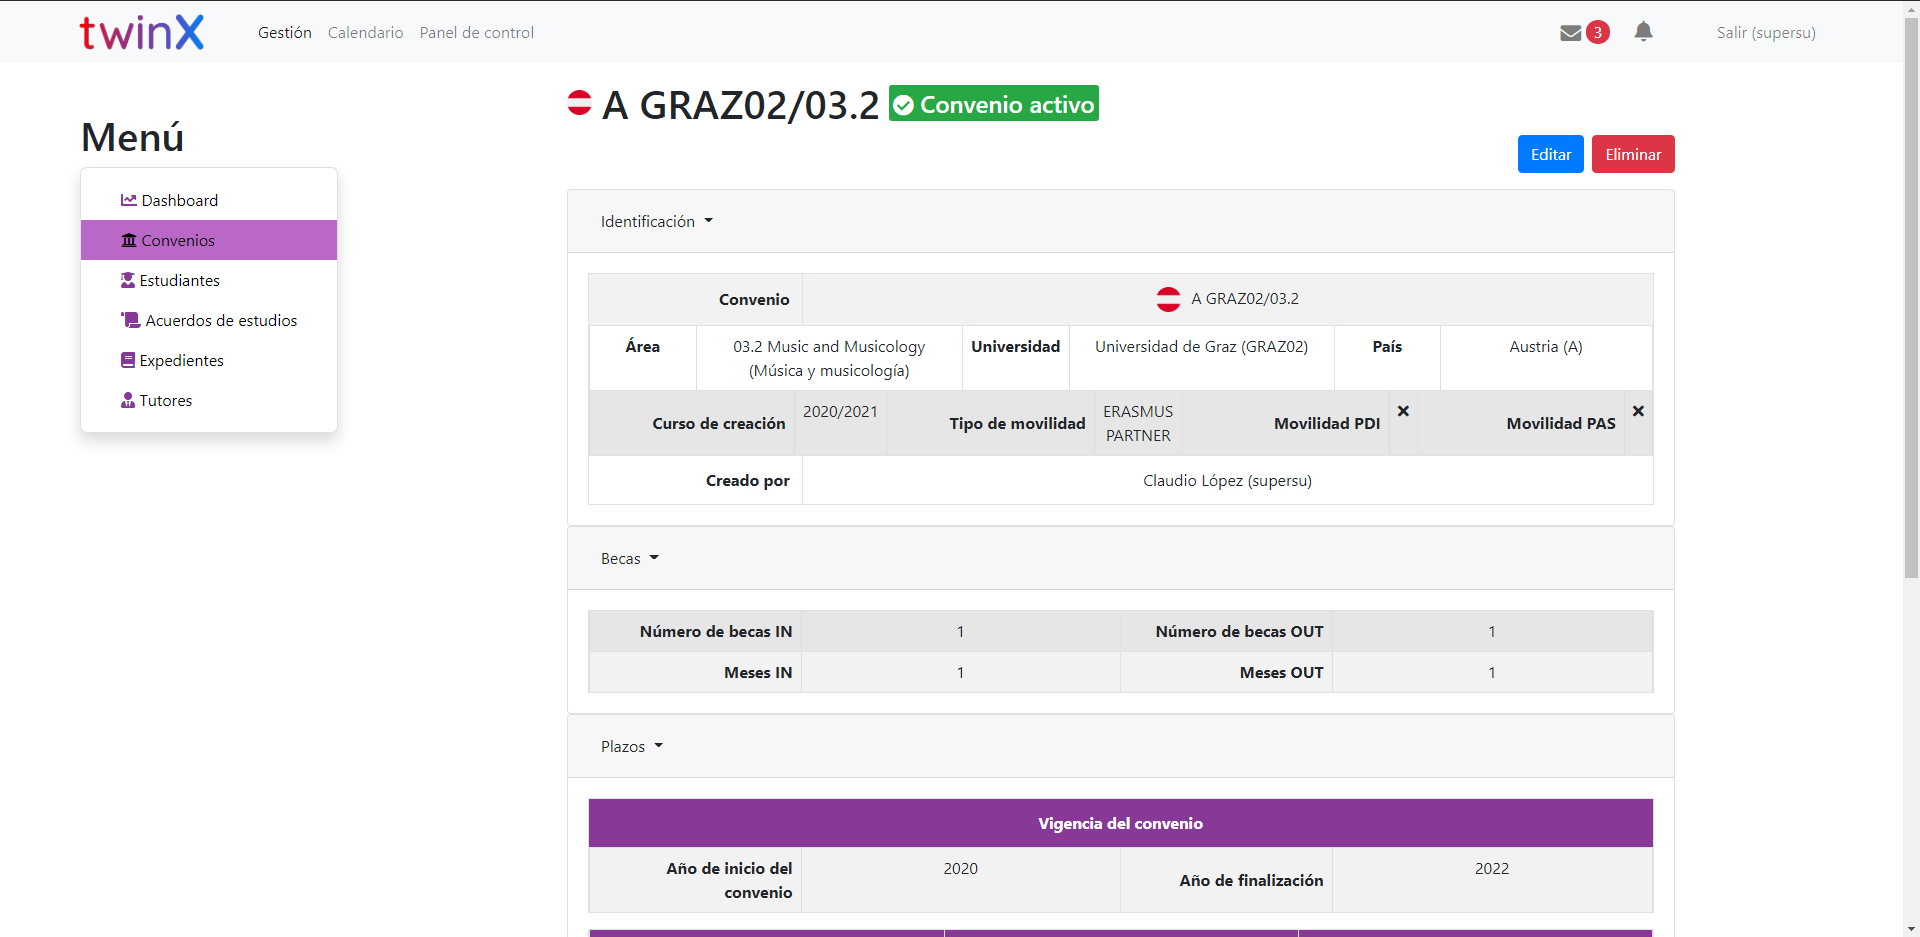
\includegraphics[width=\linewidth]{img/Capturas de twinX/vista_convenio}
	\caption{Vista de los convenios en twinX}
	\label{fig:vistaconveniotwinX}
\end{figure}


Destaca también el testigo de convenio activo, que indica si la fecha de vigencia del convenio es superior a la actual (convenio activo), si es inferior (inactivo) o si iguala al año (próxima caducidad)

\subsection{Integración del menú de estudiantes}

Respecto de los convenios, una de las cosas más destacable ya ha sido comentada: hemos necesitado ejecutar otra transacción para elegir las competencias lingüísticas de los estudiantes en su formulario (figura \ref{fig:formularioestudiantetwinX}) y para ello hemos creado una clase \texttt{EstudianteForm} que extiende a \texttt{Estudiante}.

\begin{figure}
	\centering
	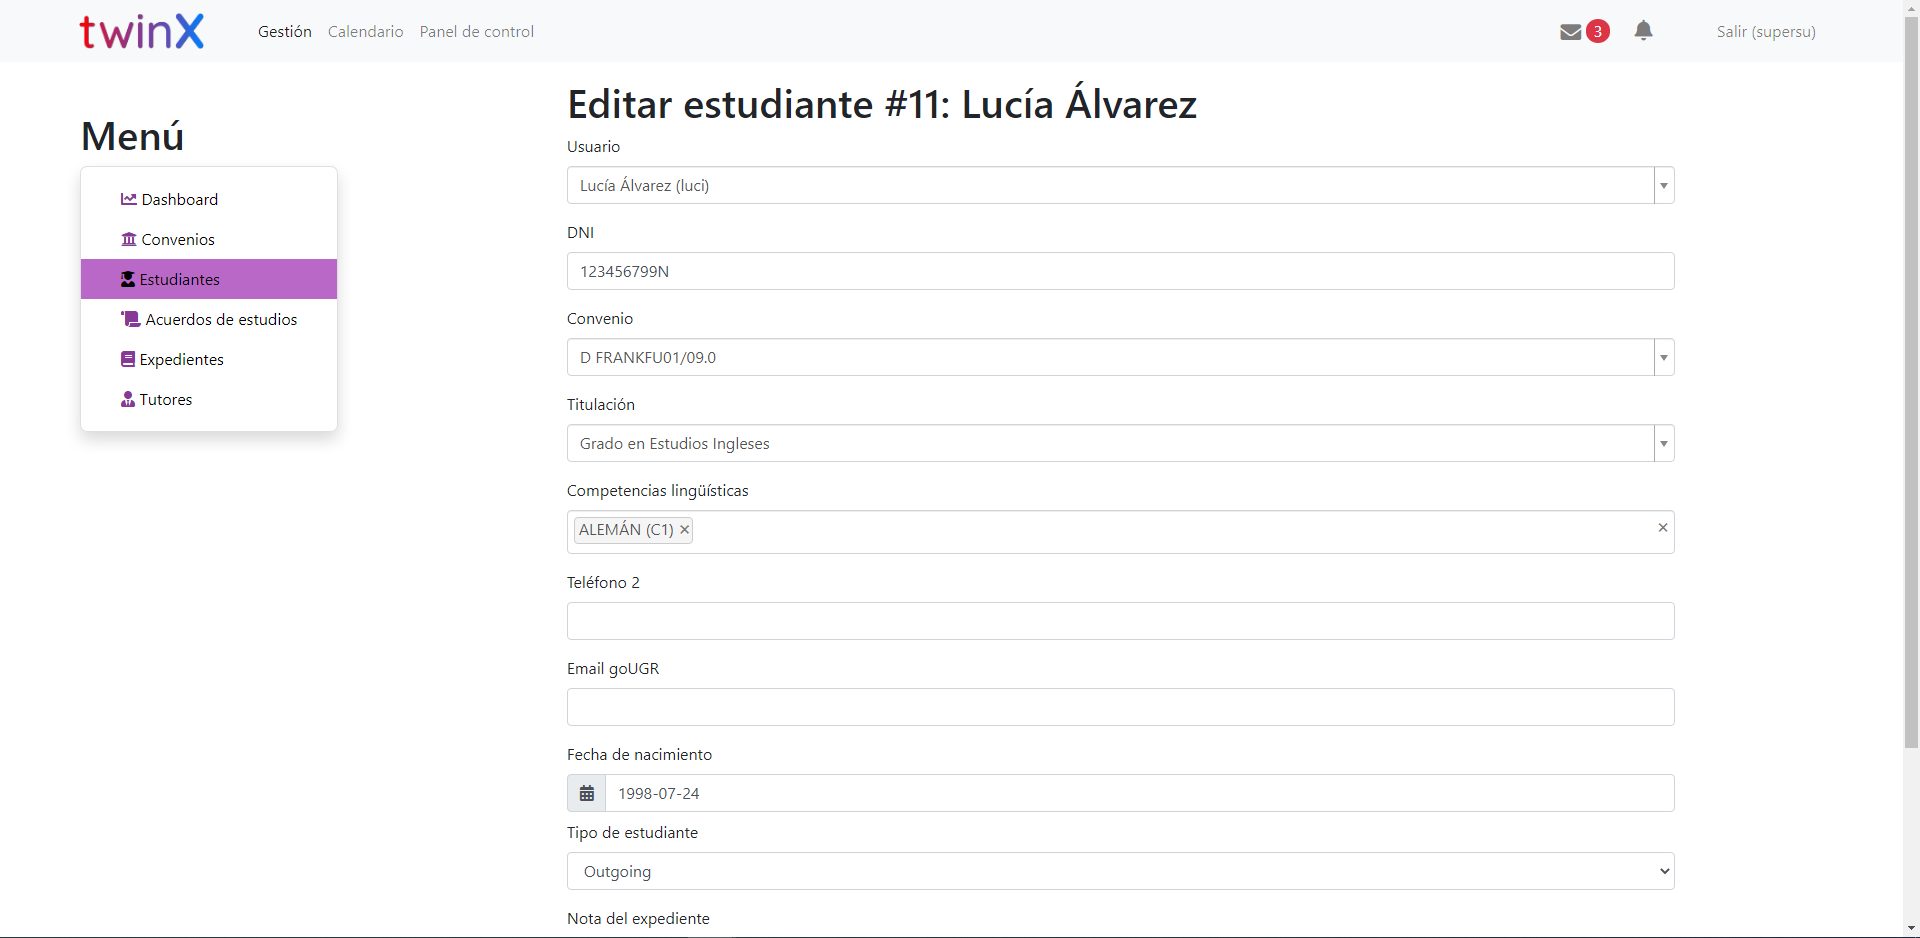
\includegraphics[width=\linewidth]{img/Capturas de twinX/formulario_estudiante}
	\caption{Creación de un estudiante en twinX}
	\label{fig:formularioestudiantetwinX}
\end{figure}

Desde el menú de estudiantes (figura \ref{fig:menuestudiantestwinX}) podemos pivotar hacia su convenio (icono verde) o hacia su acuerdo de estudios (icono turquesa). Al lado del nombre del estudiante, figura un círculo de color rojo o azul, según si es saliente o entrante, respectivamente, como apuesta de rediseño de rellenar el fondo del nombre del estudiante de uno de estos colores en TWINS según su modalidad (figura \ref{fig:alumnos}).

\begin{figure}
	\centering
	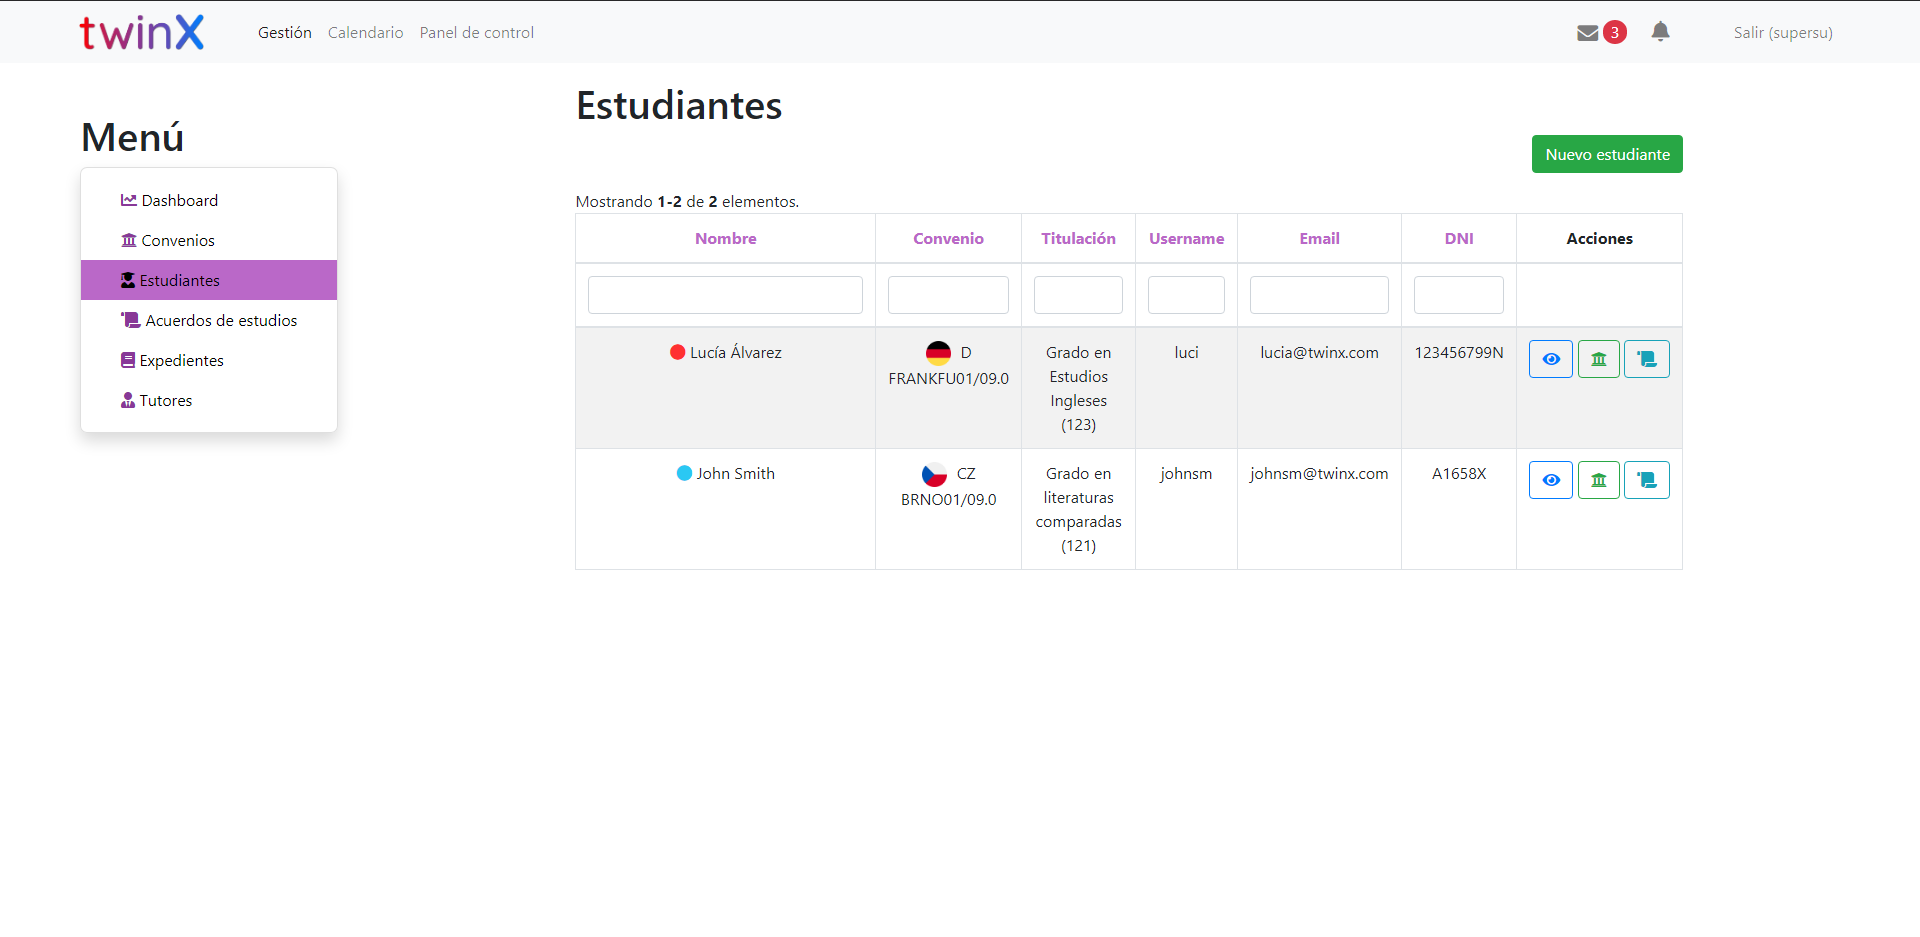
\includegraphics[width=\linewidth]{img/Capturas de twinX/menu_estudiante}
	\caption{Menú de estudiantes en twinX}
	\label{fig:menuestudiantestwinX}
\end{figure}

La vista del estudiante (\ref{fig:vistaestudiantetwinX}) también ha tenido un importante rediseño. Se ha vuelto a tener en cuenta la necesidad de tener accesos directos a demás información del usuario y respecto del boceto que creamos para esta vista (figura \ref{fig:estudiante_detalleWF}) destaca el haber prescindido del  excesivo uso de iconos que se hizo en el \textit{wireframe}, algo bastante positivo, ya que no se alcanzaba a entender bien en todos los casos a qué dato correspondía cada campo.

\begin{figure}
	\centering
	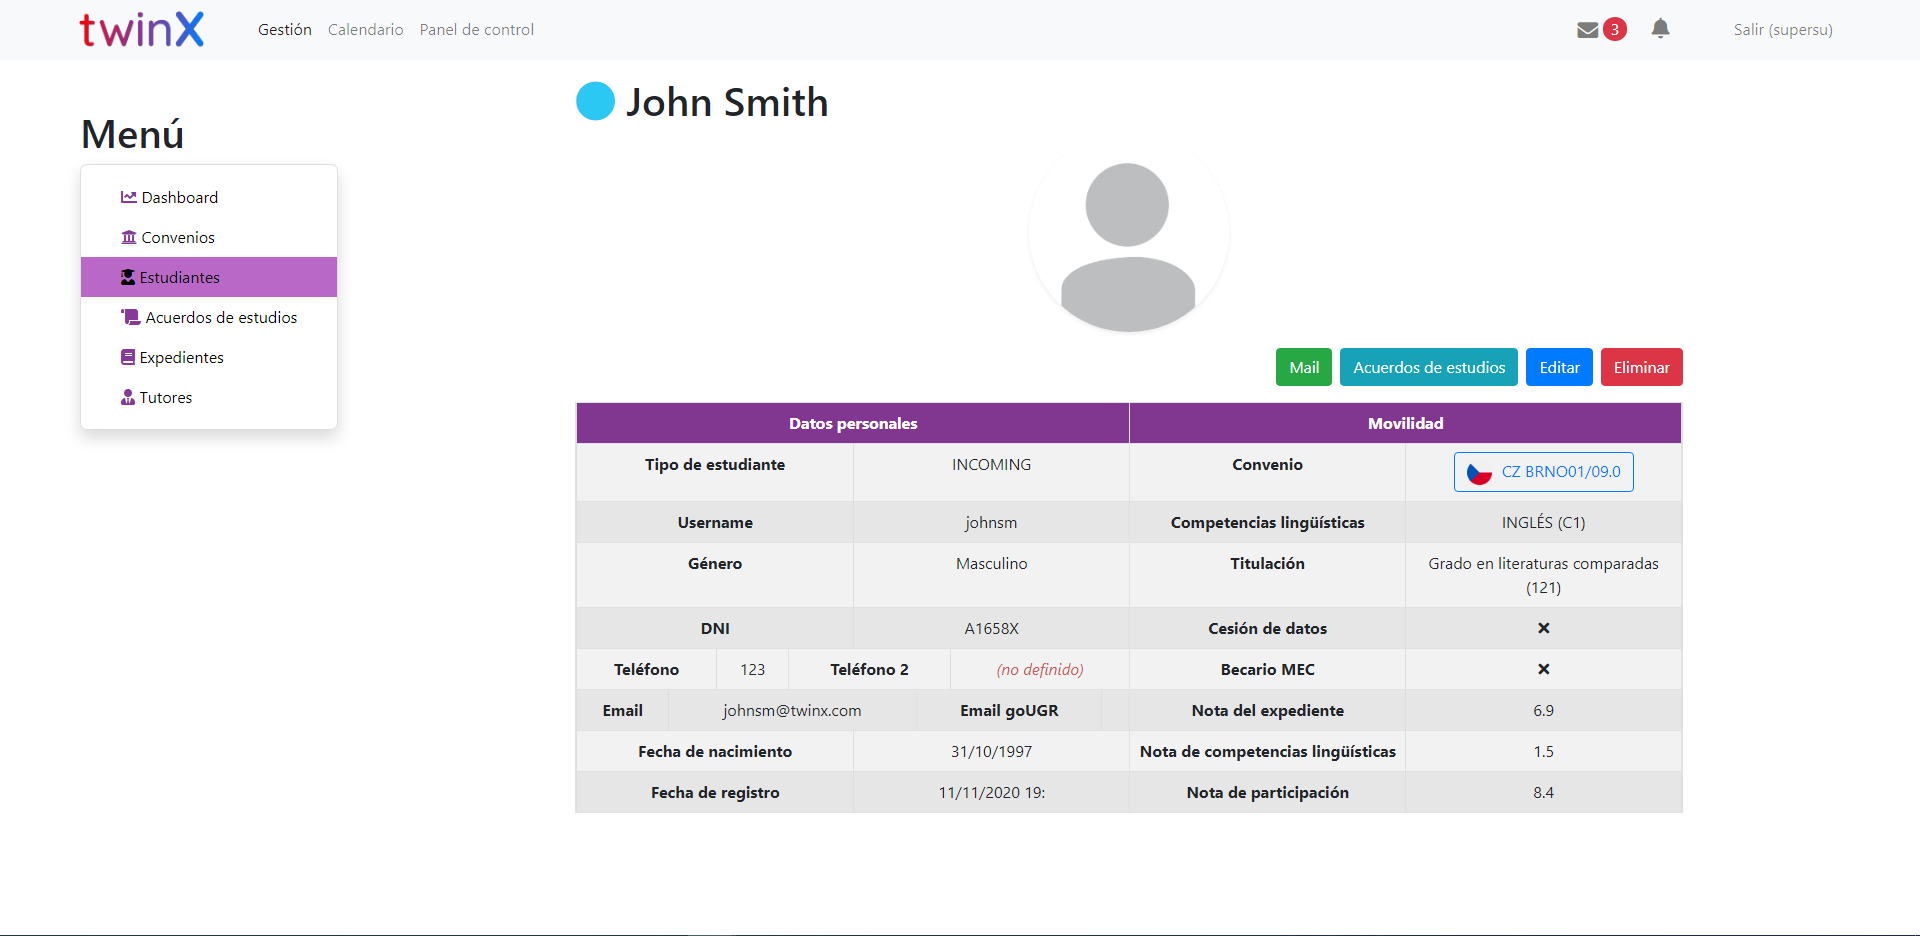
\includegraphics[width=\linewidth]{img/Capturas de twinX/vista_estudiante}
	\caption{Vista de estudiante en twinX}
	\label{fig:vistaestudiantetwinX}
\end{figure}

Llegados a este punto, señalamos la generación automática de la nota de competencia lingüística y de participación de un estudiante. En TWINS, ambas puntuaciones tenían que guardarse en dos atributos por separado, pero se ha creído conveniente desarrollar un algoritmo para el cálculo de las notas.
De acuerdo con las exigencias del convenio, si un estudiante tiene la misma competencia que se le requiere, no se le atribuye una nota extra. Sin embargo, a partir de B1 (que es lo mínimo que se puede requerir), se puede premiar con 1 punto adicional si el estudiante tiene un nivel B2, 1.5 puntos si es C1 o 2 puntos si su título es de C2, independientemente del nivel que se parta; esto es, si el estudiante tiene un C1 pero le requieren un B2 o B1, se le suman 1.5 puntos extra, y 2 puntos en caso de poseer un nivel C2 pero le requirieran C1 o inferior.

Entonces, en el modelo de \texttt{Estudiante}, el algoritmo es el siguiente:

\begin{minted}[frame=lines,breaklines]{php}
<?php
(...)
public function getNotaCompetenciaLing()
{
	$compConvenioRaw = $this->convenio->reqLingConvs;
	$compEstudianteRaw = $this->relClEsts;
	$compConvenio = [];
	$compEstudiante = [];
	$extra = 0;
	$valores = [
	'B1' => 0.5,
	'B2' => 1,
	'C1' => 1.5,
	'C2' => 2
	];
	
	foreach ($compConvenioRaw as $cC) {
		$compConvenio []= $cC->comp;
	}
	
	foreach ($compEstudianteRaw as $cE) {
		$compEstudiante []= $cE->cl;
	}
	
	foreach ($compEstudiante as $cE){
		if(in_array($cE, $compConvenio))
		unset($compConvenio[$cE->id]); // No tenemos en cuenta las competencias que requiere el convenio
	}
	
	foreach ($compEstudiante as $cE){
		foreach ($compConvenio as $cC){
			if($cE->lengua == $cC->lengua){
				if($valores[$cE->nivel] > $valores[$cC->nivel])
				$extra += $valores[$cE->nivel];
			}
		}
	}
	
	return $extra;
}

(...)
?>
\end{minted}

Entonces, el valor devuelto por el método es la nota de competencia lingüística que se muestra en la figura \ref{fig:vistaestudiantetwinX} y la nota de participación, la suma de ésta con la del expediente, ya es con esa nota con la que participa en el sorteo de las plazas de movilidad. Con este algoritmo, ahorramos un total de dos atributos en la tabla de estudiante, y teniendo en cuenta que la cantidad de registros a almacenar en el día a día es elevado, podemos considerar esta como una mejora significativa.

\subsection{Integración del menú de expedientes}

Sin pasar por el menú de acuerdos de estudios --debida la carencia de novedades respecto a todo lo ya expuesto, que se repite a lo largo del desarrollo--, entramos de lleno en los expedientes. Si bien ni el menú ni el formulario presentan características excesivamente novedosas, sí podemos encontrar un gran cambio en su vista (figura \ref{fig:vistaexpedientetwinX}).

\begin{figure}
	\centering
	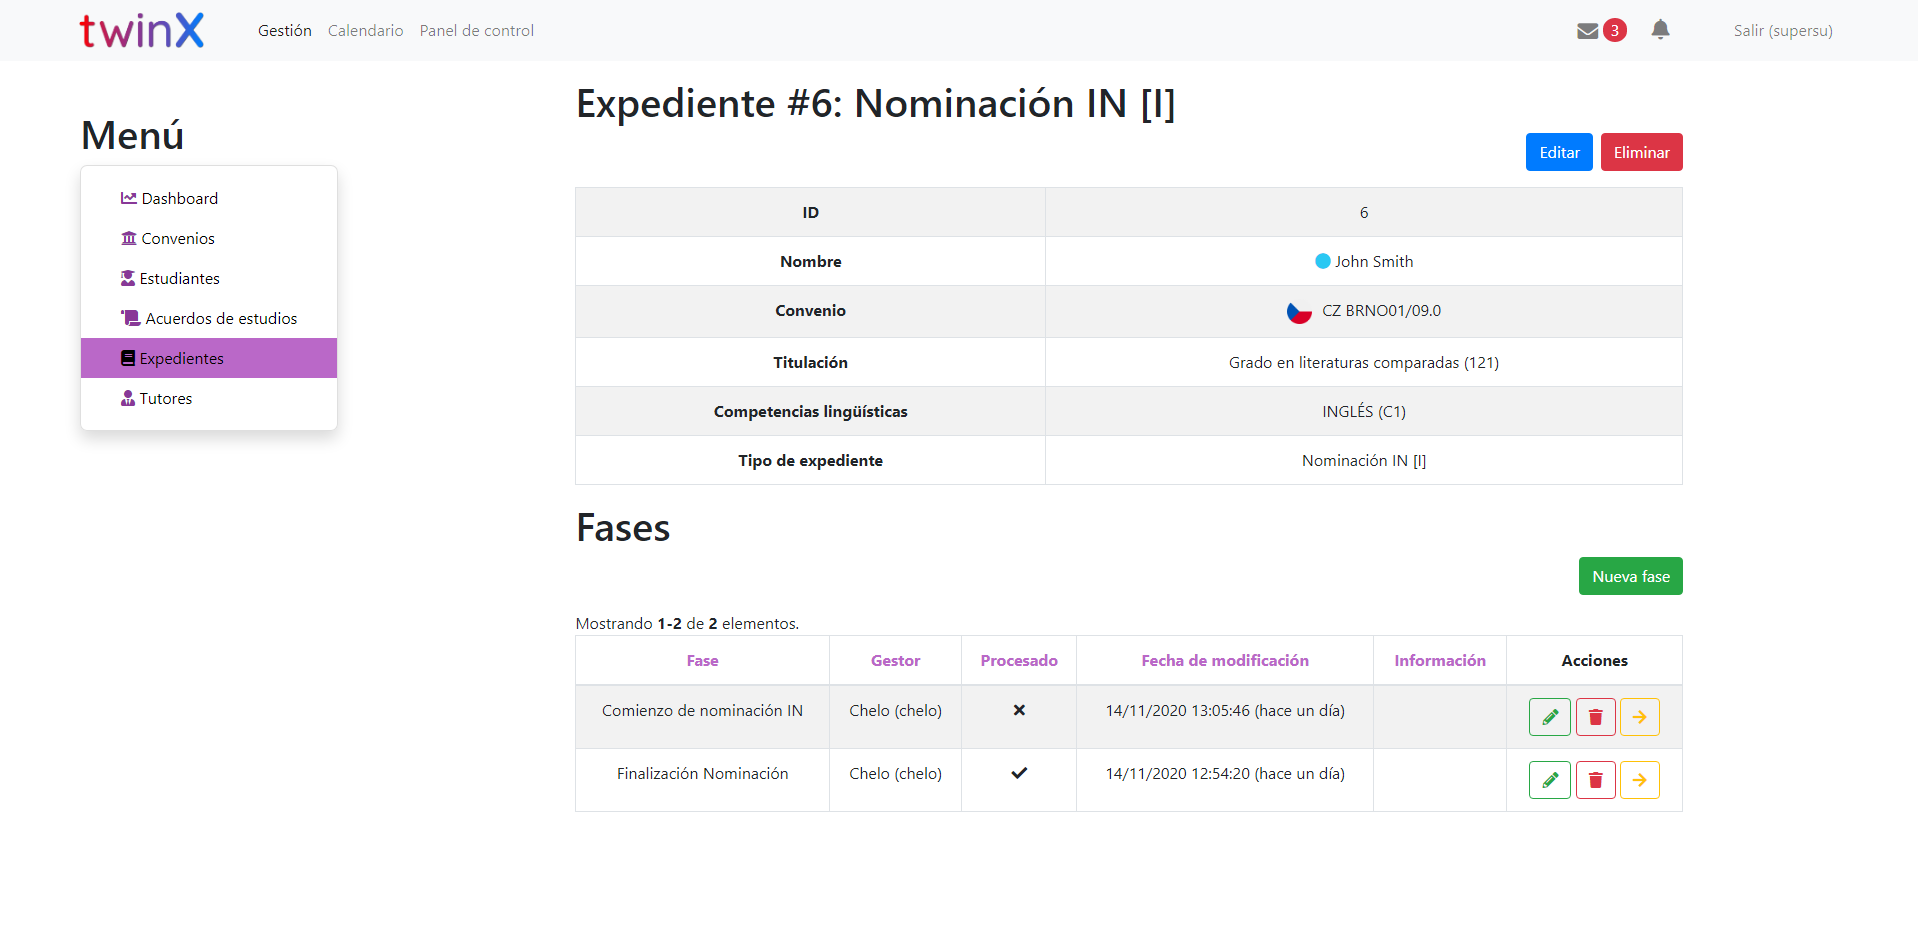
\includegraphics[width=\linewidth]{img/Capturas de twinX/vista_expediente}
	\caption{Vista de expedientes en twinX}
	\label{fig:vistaexpedientetwinX}
\end{figure}

Un expediente puede ser el de la nominación de un estudiante \textit{incoming}, y en todo momento necesitamos conocer en qué parte del proceso se encuentra su nominación. Recordemos que esto se posibilitaba con las \glspl{FaseExpedientetwinX}, y que cada una de ellas implicaba un envío de correos electrónicos en su \textbf{procesamiento}. Pues bien, al igual que en TWINS, lo más oportuno es ver el expediente del estudiante y su situación actual, con un historial de todo lo ya ocurrido en dicho registro. Esto lo hemos hecho posible embebiendo un menú en la interfaz de la vista del expediente; en este caso, aunque pueda pensarse que es el de la tabla \texttt{fase\_expediente}, en realidad se trata del de \texttt{rel\_fase\_exp} (relación de fase con expediente), donde se guarda información de la fase con respecto del expediente. De este último, aclaremos que en su tabla en la base de datos no se almacena otra información que la relación de un acuerdo y un tipo de expediente.

En este caso, aunque utilicemos la librería de JavaScript \textbf{AJAX} (integrada en Yii como \textbf{Pjax}), necesitamos crear vistas compuestas; esto es, vistas que mantengan la información del expediente en la parte de arriba mientras que en la parte de abajo se pueda estar renderizando el formulario de una fase o el menú que muestra todas las fases de un expediente. Estas dos últimas son las únicas posibilidades de variación de la interfaz que comentamos, pero volviendo al \textit{modus operandi} de Yii, recordemos que crear y actualizar son dos acciones distintas a ojos del controlador, aunque ambas usen el mismo formulario. Por tanto, necesitaremos los siguientes elementos:

\begin{itemize}
	\item \textbf{\texttt{\_view.php}}: donde almacenaremos la vista compartida y persistente de \texttt{Expediente}.
	\item \textbf{\texttt{view.php}}: la vista predeterminada con la información del expediente y sus fases.
	\item \textbf{\texttt{view-new-fase.php}}: carga la vista del expediente y el formulario de creación de una nueva fase.
	\item \textbf{\texttt{view-update-fase.php}}: carga la vista del expediente y el formulario de modificaicón de una fase ya existente.
\end{itemize}

Dentro de las tres últimas, llamamos a una instancia del controlador \\ \texttt{RelFaseExpController.php} desde el que se llama al menú, al creador y al actualizador respectivamente, en sus métodos \texttt{action} correspondientes:

\begin{minted}[frame=lines]{php}
	<?php include('_view.php') ?>
	
	<?= $relExpFase->actionCreate($model) ?>
\end{minted}

Ya que en las tres vistas se precisa de una instancia del controlador, es en \texttt{\_view.php} donde se sitúa la creación de la misma:

\begin{minted}[frame=lines, breaklines]{php}
<?php
(...)

$relExpFase = new \backend\modules\gestion\controllers\RelExpFaseController('rel-exp-fase', Yii::$app->getModule('rel-exp-fase'));

(...)
?>
\end{minted}

Entonces, dado que es al controlador de \texttt{Expediente} al que se llama para cargar las distintas vistas compuestas (ya que nos situamos en \texttt{localhost/gestion/expediente}), es él mismo quien tiene que orquestar las llamadas a los métodos \texttt{action} para cargarlas, por lo que tenemos que crear acciones nuevas que llamen a los archivos de vista nuevos. A su vez y en aras de reutilizar código, éstos métodos harán una llamada a \texttt{actionView}, que es el mismo método que carga la vista del expediente, pero con nuevos parámetros, para que podamos enlazar el flujo de control con \texttt{RelExpFaseController.php}.

Una vez llegada la ejecución a uno de los archivos que permiten crear o modificar una fase para el expediente, se llama al método \texttt{actionCreate} o \texttt{actionUpdate} de \texttt{RelExpFase.php}, pero con una novedad: se pasa como argumento el \texttt{Expediente} actual que, por tanto, el formulario ya tiene que llevar relleno en el campo destinado a ello. Lo mismo pasa con la actualización. En el caso de la vista de la lista de las fases de un expediente (archivo por defecto \texttt{view.php}), también se necesita el ID del expediente que se visualiza, para devolver tan solo aquellas fases pertenecientes al mismo. Esto se consigue modificando el método \texttt{actionIndex} de \texttt{RelExpFaseController.php} de la siguiente forma:

\begin{minted}[frame=lines, breaklines]{php}
<?php
(...)

public function actionIndex($idExpediente = false)
{
	$path = '';
	$query = RelExpFase::find();
	
	if($idExpediente) {
		$path = '@backend/modules/gestion/views/rel-exp-fase/';
		$query = $query->where(['id_exp' => $idExpediente]);
	}
	
	
	$dataProvider = new ActiveDataProvider([
	'query' => $query,
	]);
	
	return $this->render($path . 'index', [
	'dataProvider' => $dataProvider,
	'idExpediente' => $idExpediente,
	]);
}

(...)
?>
\end{minted}

Los métodos \texttt{actionCreate} y \texttt{actionUpdate} tienen una implementación similar. Nótese que no hemos impedido el funcionamiento corriente de los métodos, sino que los hemos complementado con atributos que poseen valores por defecto porque no siempre tienen que requerirse, en caso de necesitar hacer uso de la interfaz de forma independiente a la vista de expedientes como aquí se necesita. Toda esta estructura se tiene también para la visualización de los correos (\texttt{MailPredefinido}) que se envían en cada fase en el módulo del panel de control, cuya implementación es similar y por ello, no la hemos tratado.


\subsection{Integración del dashboard}

De nuevo, poco hay que decir sobre la implementación del menú de tutores, y por ello, pasamos a una de las grandes novedades que supone twinX sobre TWINS: la vista de dashboard (figura \ref{fig:dashboardtwinX}). Su objetivo no es otro que el presentar la información de mayor relevancia al usuario en cuanto abra la aplicación. Esta facilidad se ofrecía en TWINS en la forma de tres menús que bloqueaban toda la pantalla, ofreciendo información sobre el calendario, los avisos (mensajes en nuestro caso) y expedientes sin procesar, obligando al usuario a salir de las tres pantallas hasta llegar al menú principal. De esta manera, la aparición del dashboard no es bloqueante, y con tan solo una vista se resumen todos los asuntos que precisan de la atención del gestor al arrancar twinX.

\begin{figure}
	\centering
	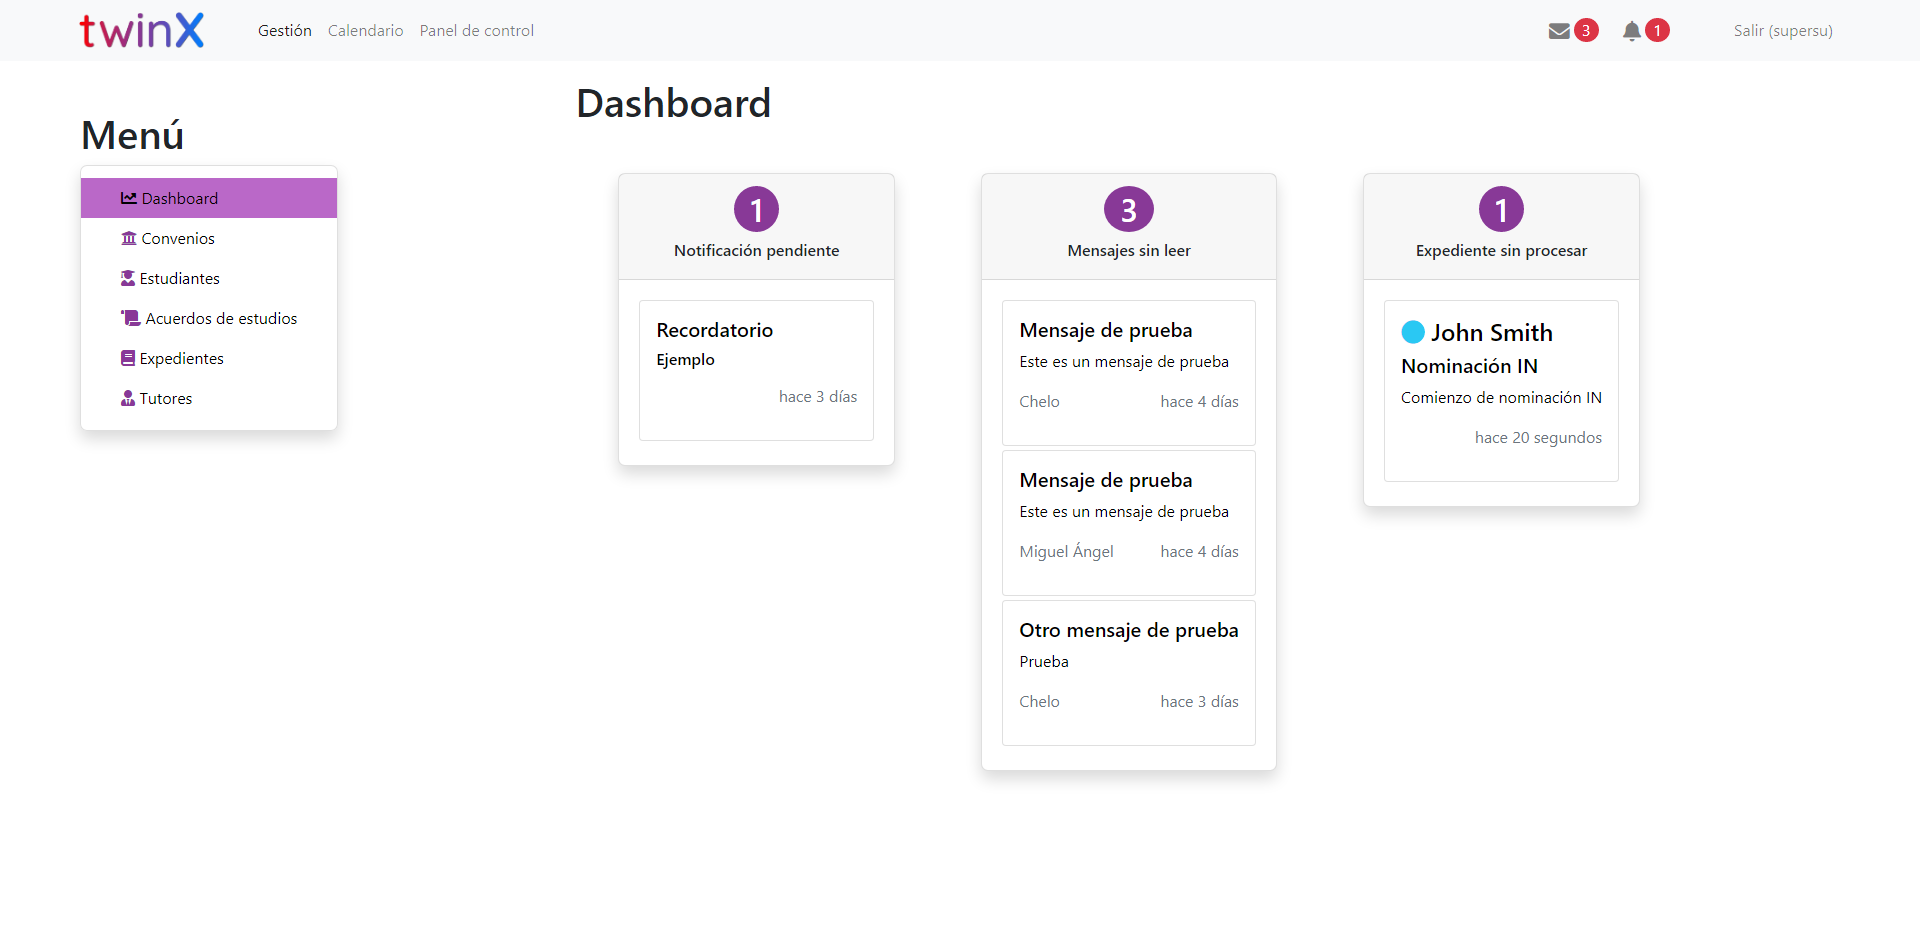
\includegraphics[width=\linewidth]{img/Capturas de twinX/dashboard}
	\caption{Dashboard de twinX}
	\label{fig:dashboardtwinX}
\end{figure}

En este caso, no ha sido necesaria la creación de ningún menú CRUD ni ningún modelo nuevo. Simplemente hemos creado la vista \texttt{dashboard.php} en su directorio (\texttt{backend/modules/gestion/views/dashboard}) y en la carpeta de controladores, el \texttt{DashboardController.php}, poseedor de tan solo un método \texttt{actionIndex} que carga el archivo de la vista.

Dejando aparte las cuestiones de estilo, la información puede mostrarse a través de consultas a los demás modelos ya creados. Como mejora adicional, aunque aún no hayamos hablado de los mensajes y los recordatorios aún, vamos a presentar la última clase especial que tiene un gran potencial en Yii y de la cual hemos hecho uso en la implementación del dashboard. Son las clases \textbf{\texttt{Query}}. En ellas, cualquier método que se cree, puede ser ejecutado a modo de QBE a la hora de hacer una consulta a la base de datos, de modo que podamos ahorrar y reutilizar código. Por ejemplo, este es el método \texttt{notificaciones} de \texttt{RecordatorioQuery.php}:

\begin{minted}[frame=lines]{php}
<?php
(...)

public function notificaciones($db = null)
{
	return Recordatorio::find()
	->where(['id_usr_aviso' => Yii::$app->user->id])
	->andWhere(['<>', 'completado', '1'])
	->andWhere(['<', 'deadline', date('yy-m-d H:i')]);
}

(...)
?>
\end{minted}

Es sencillo, pero dado que en el dashboard necesitamos trabajar con las notificaciones pendientes en dos ocasiones (extraer el número de recordatorios pendientes y su vista de detalle en la sección de notificaciones), es muy práctico tenerlo para llamarlo de la siguiente manera:

\begin{minted}[frame=lines,breaklines]{php}
	<?php
	(...)
	
	$notificaciones = \common\models\Recordatorio::find()->notificaciones();
	
	(...)
	
	foreach ($notificaciones->with('emisor')->all() as $notificacion) {
		echo '<div class="card p-3 notificacion-dashboard mb-1">';
		$output = '<h5>Recordatorio</h5>';
		$output .= '<h6>' . $notificacion->titulo . '</h6> ';
		$output .= '<p>' . $notificacion->descripcion . '</p>';
		$output .= '<p class="text-muted d-flex flex-row-reverse">' . Yii::$app->formatter->asRelativeTime($notificacion->timestamp) . '</p>';
		echo \yii\helpers\Html::a($output, ['/calendario/recordatorio/view', 'id' => $notificacion->id]);
		echo '</div>';
	}
	
	(...)
	?>
\end{minted}

Es decir, en \texttt{\$notificaciones} almacenamos la \textit{query}, y la usamos llamando al método \texttt{count()} para obtener el número de registros o el array con todas ellas (\texttt{all()}) si necesitamos trabajar con cada una de ellas por separado.

En última instancia, es interesante también considerar la mejora que presenta la introducción de secuencias \texttt{with(<atributo>)}. Al especificar el \texttt{atributo} del modelo de la clase para la que se hace la consulta, se está evitando a toda costa lo que se conoce como el fenómeno de la «carga perezosa» o \textit{lazy loading}. Por ejemplo, para la carga de los expedientes sin procesar utilizamos varias sentencias \texttt{with} que nos permiten almacenar el contenido del atributo que se especifica, evitando posteriormente el tener que hacer consultas adicionales:

\begin{minted}[frame=lines,breaklines]{php}
	<?php
	foreach ($expedientes->with('exp')->with('exp.ae')->with('fase')->all() as $expediente) {
		echo '<div class="card p-3 notificacion-dashboard mb-1">';
		$output = '<h4>' . $expediente->exp->ae->estudiante->nombreEstudiante . '<h4>';
		$output .= '<h5>' . $expediente->exp->tipoExp->descripcion . '</h5> ';
		$output .= '<p>' . $expediente->fase->descripcion . '</p>';
		$output .= '<p class="text-muted d-flex flex-row-reverse">' . Yii::$app->formatter->asRelativeTime($expediente->timestamp) . '</p>';
		echo \yii\helpers\Html::a($output, ['/gestion/expediente/view', 'id' => $expediente->id_exp]);
		echo '</div>';
	}
	?>
\end{minted}

Es decir, como tenemos que recuperar atributos del acuerdo de estudios (\texttt{ae}) de \texttt{exp} y la \texttt{fase}, podemos ordenar que se almacenen los valores para no tener que recuperarlos de nuevo. Este comportamiento recibe el nombre de «carga entusiasta» o \textit{eager loading}. Más específicamente, sin ninguna orden \texttt{with} en toda la vista del dashboard, tendríamos un total de 45 \textit{queries}, mientras que con todas ellas, rebajamos el número hasta 38.

\subsection{Integración de la mensajería}

Por último en este módulo, hemos implementado la mensajería de twinX (figura \ref{fig:bandejaentradatwinX}). En lugar de tener un \texttt{actionIndex} en \texttt{MensajeController.php} general para la lista de mensajes, se ha sustituido por un \texttt{actionRoute}, que diverge la vista del menú en bandeja de entrada o elementos enviados y carga los mensajes que mostrar en función de si se es emisor o receptor de los mismos:

\begin{minted}[frame=lines]{php}
<?php
(...)
public function actionRoute($bandeja)
{
	$searchModel = new MensajeSearch();
	$query = $searchModel->searchQuery(Yii::$app->request->queryParams);
	
	if($bandeja == 'INBOX')
		$query->andWhere(['id_receptor' => Yii::$app->user->id]);
	else
		$query->andWhere(['id_emisor' => Yii::$app->user->id]);
	
	$dataProvider = $searchModel->search($query);
	
	return $this->render('index', [
		'searchModel' => $searchModel,
		'dataProvider' => $dataProvider,
		'bandeja' => $bandeja
	]);
}
(...)
?>
\end{minted}


\begin{figure}
	\centering
	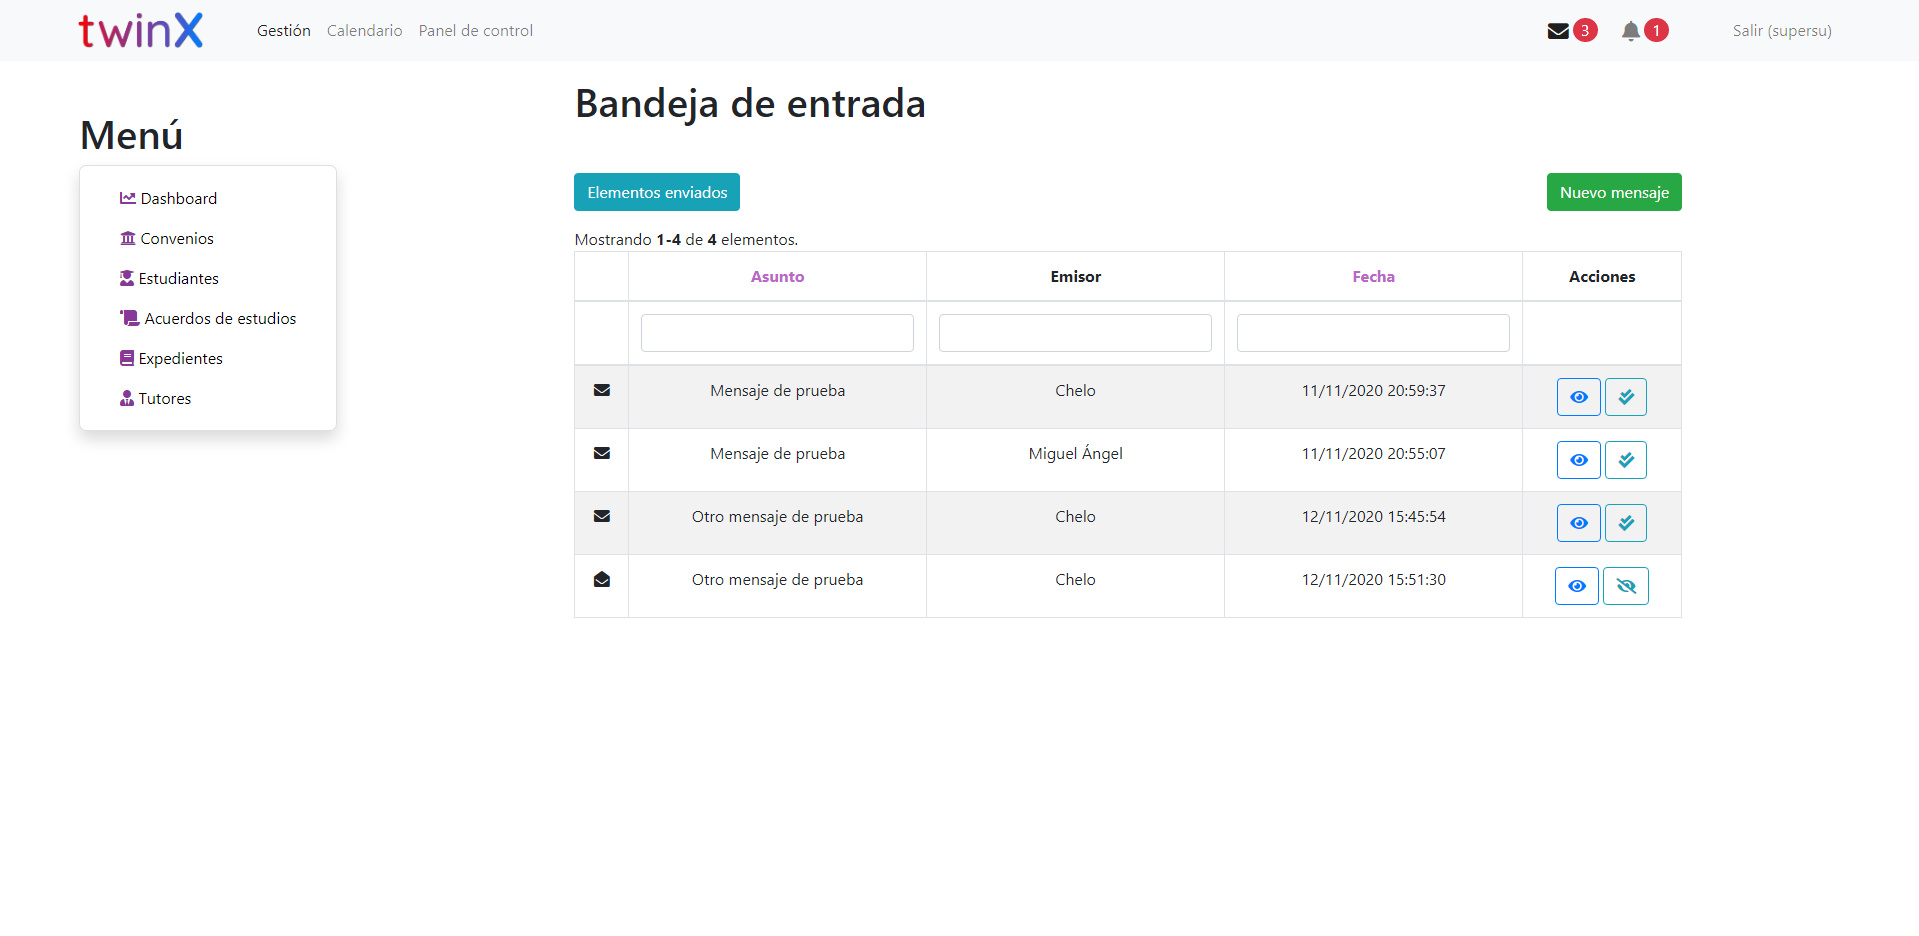
\includegraphics[width=\linewidth]{img/Capturas de twinX/bandeja_entrada}
	\caption{Bandeja de entrada en twinX}
	\label{fig:bandejaentradatwinX}
\end{figure}

De la vista de menú, se ha creído conveniente crear un pequeño atajo para marcar un mensaje como leído o no leído. También se ha tratado de simplificar la vista (figura \ref{fig:vistamensajetwinX}) condensando los atributos de valor de un mensaje en su cabecera y su asunto como título del contenido. Destaca también la ausencia de opciones como la edición y eliminación de un mensaje ya enviado, para mantener el significado de la entidad \texttt{Mensaje} y no tratarla como una tupla más de una tabla en base de datos.

\begin{figure}
	\centering
	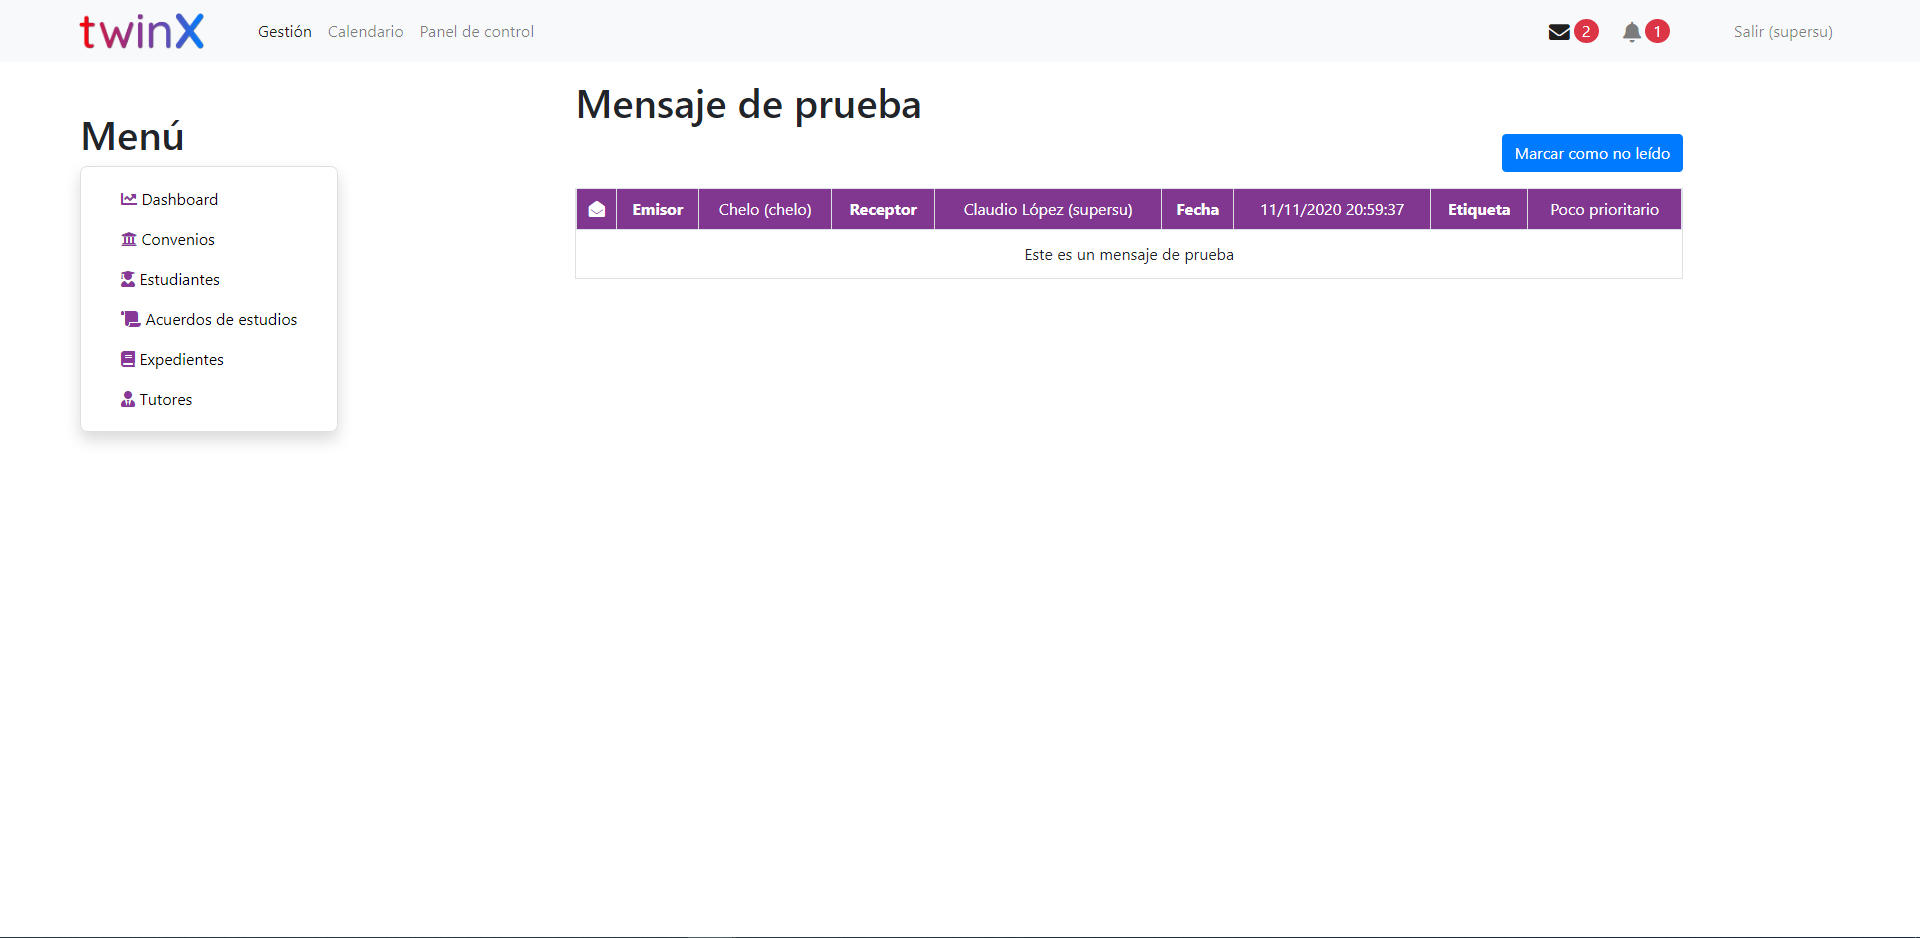
\includegraphics[width=\linewidth]{img/Capturas de twinX/vista_mensaje}
	\caption{Vista de mensaje en twinX}
	\label{fig:vistamensajetwinX}
\end{figure}


\section{Desarrollo del módulo de calendario}

La parte del calendario en TWINS podía resultar un poco confusa al tratar de entender cómo funciona: un calendario con eventos comunes a todo el mundo. Estos eventos con un máximo de dos personas a las que poder avisar, tenían la capacidad de encontrar asociadas numerosas tareas que dividían el evento en distintas etapas. Las tareas, a su vez, contaban con otro máximo de dos personas a las que poder asignar esa tarea y con una fecha límite concreta. Tenían características incluso como la atribución de un porcentaje de progresión en la completitud de la tarea o también el evento (figura \ref{fig:nuevatarea}).

En el boceto de la figura \ref{fig:nuevo_eventoWF} representamos una aproximación a lo que podría ser el calendario en twinX, pero aunque quizás no tan complicado de implementar, su desarrollo necesita bastante tiempo, ya que en twinX, de acuerdo con el modelo de la base de datos (figura \ref{fig:modeloBD}), se tenía una relación muchos a muchos para poder avisar a cuantos gestores se quisiera para un evento o una tarea creados. Esto complica la implementación, haciéndola menos inmediata e inteligible, pues pensemos que tendríamos que desempeñar de nuevo las mismas acciones que para generar vistas compuestas; en este caso, varias tablas CRUD embebidas, unas dentro de otras.

Ya hemos demostrado que es posible hacer este tipo de direccionamiento de los flujos de información para obtener los resultados que se quieren, pero por motivos de tiempo, se ha decidido cambiar la implementación de esta parte por otra, dentro del módulo del calendario, ya que no afecta a la consecución de los objetivos generales del proyecto. Más concretamente, al comienzo del segundo sprint (\ref{subsubsec:segundosprint}), se tomó la decisión de dejar fuera de la programación la \hyperref[tab:HU3.1]{HU3.1} y la \hyperref[tab:HU3.2]{HU3.2}. En consecuencia, se pudo llevar a cabo el desarrollo de la \hyperref[tab:HU3.3]{HU3.3} y la \hyperref[tab:HU4]{HU4} con más amplio margen temporal y con la posibilidad de establecer un mayor enfoque en los resultados y la calidad de los mismos con respecto, como siempre, a los objetivos generales del proyecto.

Sobre la codificación de esta parte, las tareas a realizar eran similares: creación de un módulo, generación del modelo de \texttt{Recordatorio} y del menú CRUD para el mismo. Hemos, sin embargo, filtrado la aparición de recordatorios en el menú principal (figura \ref{fig:recordatoriostwinX}) a tan solo los que crea el usuario. Cabe destacar que un gestor puede dirigir recordatorios a otro compañero, por lo que le aparecerán en su menú. Sin embargo, si otro usuario crea un recordatorio para nosotros, no lo veremos ahí, sino en la sección de notificaciones, que tiene también un testigo rojo a modo de contador en la cabecera de la web para que nos demos cuenta siempre que tengamos alguno pendiente. También aparecen en el dashboard, por lo que al abrir la aplicación no solo veríamos que tendríamos un recordatorio pendiente, sino que también podríamos apreciar de qué se trata. Si hacemos clic en él, nos redirigirá a la vista de detalle, muy similar a la de los mensajes. Una vez se marcan como completados, desaparecerán de notificaciones.

\begin{figure}
	\centering
	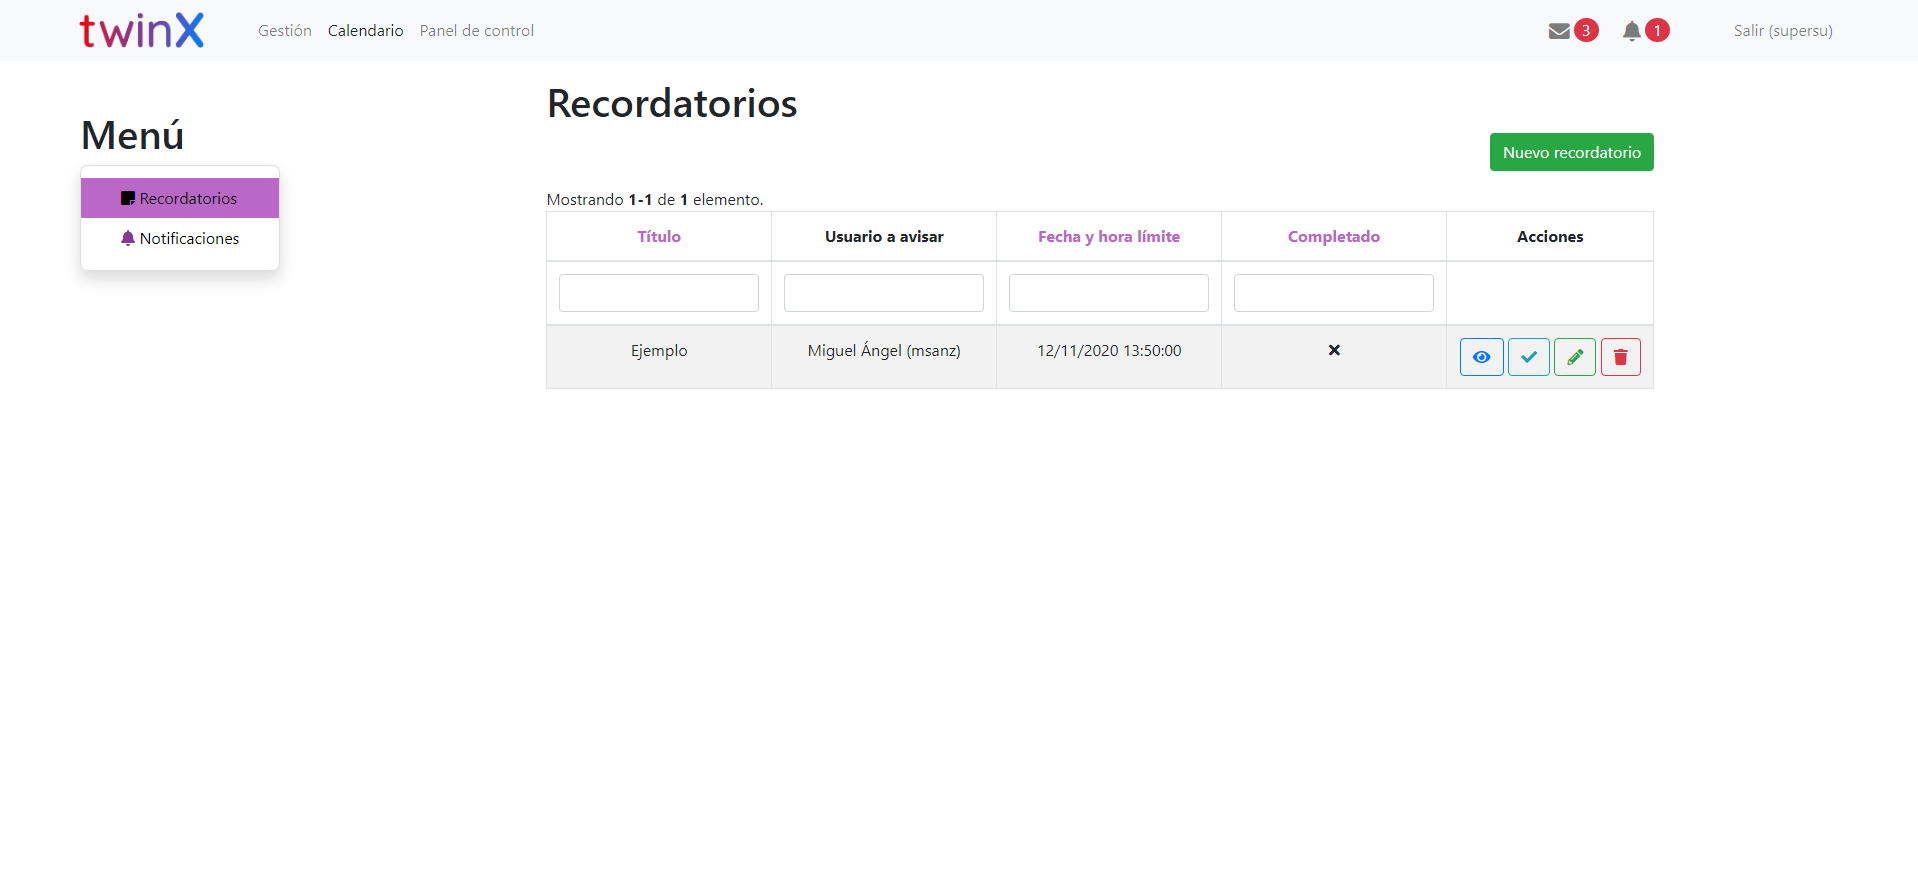
\includegraphics[width=\linewidth]{img/Capturas de twinX/recordatorios}
	\caption{Menú de recordatorios en twinX}
	\label{fig:recordatoriostwinX}
\end{figure}

Para las notificaciones no nos ha hecho falta crear otro modelo, tan solo una vista y un controlador sencillos, al igual que para el dashboard, ya que las consultas que se hacen a la base de datos se realizan sobre instancias de modelos ya creados. Retomemos la utilidad de haber construido el método en \texttt{RecordatorioQuery.php} para recuperar todos los recordatorios pendientes para explicar el funcionamiento de \texttt{actionIndex} en \texttt{NotificacionesController.php}; ahorramos aún más código:

\begin{minted}[frame=lines]{php}
<?php
(...)

class NotificacionesController extends \yii\web\Controller
{
	public function actionIndex()
	{
		$dataProvider = new ActiveDataProvider([
		'query' => Recordatorio::find()->notificaciones()
		]);
		
		return $this->render('index', [
		'recordatorios' => $dataProvider
		]);
	}
}

?>

\end{minted}

A modo de resumen, podemos elaborar el diagrama de paquetes de la figura \ref{fig:diagramapaquetes} para ver la disposición de los archivos del proyecto en sus paquetes y directorios y la interacción entre los mismos. Se ha omitido el contenido de cada uno de los subdirectorios de \texttt{views} por motivos de extensión del diagrama, al igual que de los directorios \texttt{query} y \texttt{search}, que no aportan nombres de clases nuevas.

\begin{figure}
	\centering
	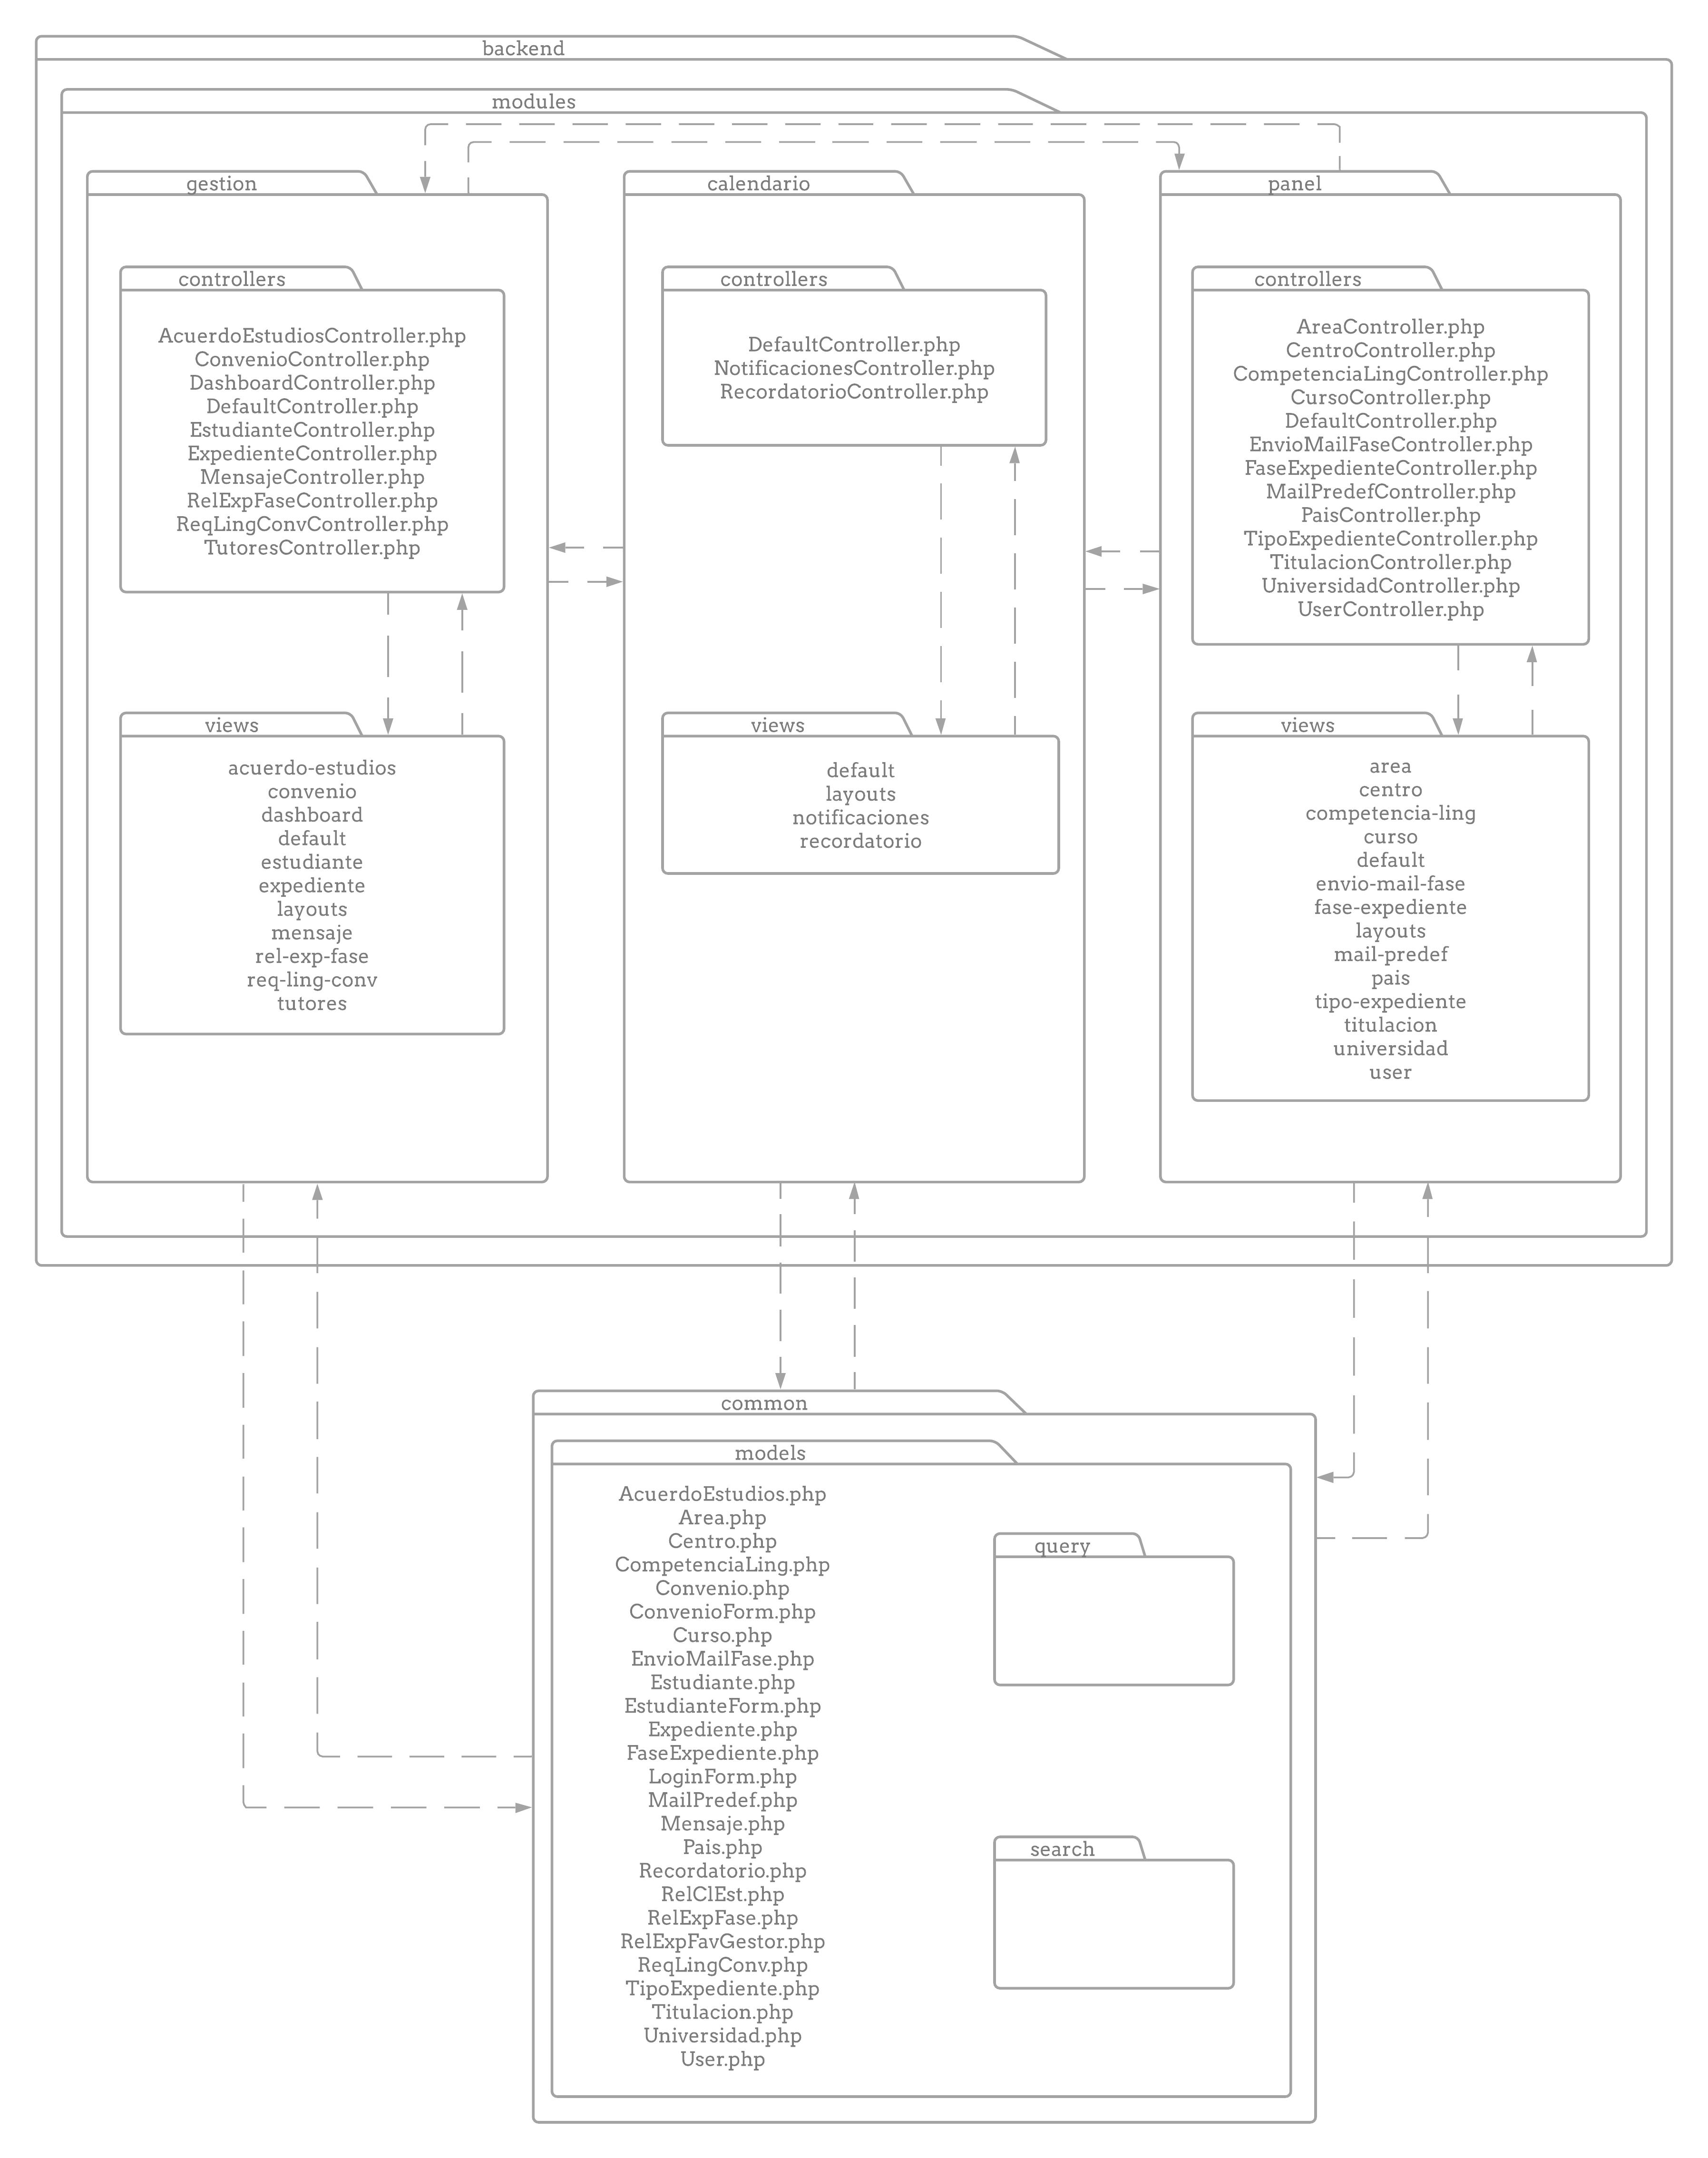
\includegraphics[width=\linewidth]{img/diagrama_paquetes}
	\caption{Diagrama de paquetes de twinX}
	\label{fig:diagramapaquetes}
\end{figure}